\documentclass[../main.tex]{subfiles}

\begin{document}
\chapter{Proposed Design}
Introduction Paragraph
\section{Airship}
The airship design provided is for reference only as Dr. Lanteigne will be proceeding with his preferred design. The airship features hemispheres at each end, a cylinder attached to the front hemisphere and a cone bridging the gap from the cylinder to the other hemisphere. The length of any section of the airship is limited to 5ft as that is the width of Dr. Lanteigne's roll. The airship will feature fixed fins for stability during forward flight. An artist's rendition of the airship can be seen in Figure ref{fig:?????????????}.
\section{Gondola}
The gondola sub-assembly is the most distinguishable feature of the airship design. The gondola moves along the keel in order to rapidly pitch the airship. The assembly can be seen in  Figure \ref{fig:gondolaIsomeric}. Movement along the gondola is driven by two friction wheels which interface with the cover on the keel through the friction between the two surfaces. Bearings are used as wheel to hold the gondola on top of the keel, while the friction wheel are in contact with the bottom edge of the keel. The gondola is comprised of two half sections which each house components, such as the battery, flight controller, transmitter, GPS module and two ESCs. Figure \ref{fig:gondolaPartialSection} shows how these components are  nested one of the gondola sections. Joining the two sections is a hinge, seen in Figure  \ref{fig:gondola1ExplodedView}, which allows the gondola to bend in the centre. The hind has a flanged end and a cap that relies upon an interference fit to ensure the gondola does not slip of the hinge axially. The bend in the middle allows the gondola to overcome a more significant turning radius compared to being fixed in a straight line, which is depicted in Figure \ref{fig:gondolaBent}. Similarly to curve fitting, the more points that are used, the better fit. Braking of the gondola is accomplished by turning the friction wheels in the opposite direction and the position is held by a linear actuator, which provides force perpendicular to the keel surface. The linear actuator motion can be seen in Figure \ref{fig:linearActuatorAndMotor}. The gondola has been designed to be resistant to small amounts of water, considering the gondola will always be shielded from rainfall by the envelope, therefore total waterproofing is not required. Cable glands will be used for all surfaces perpendicular to rainfall that require waterproofing. They can be seen in Figure \ref{fig:gondola1ExplodedView}. The gondola section are made using high quality 3D prints, given their complex geometries and relatively small size.
\\

\begin{figure}[H]
	\centering
	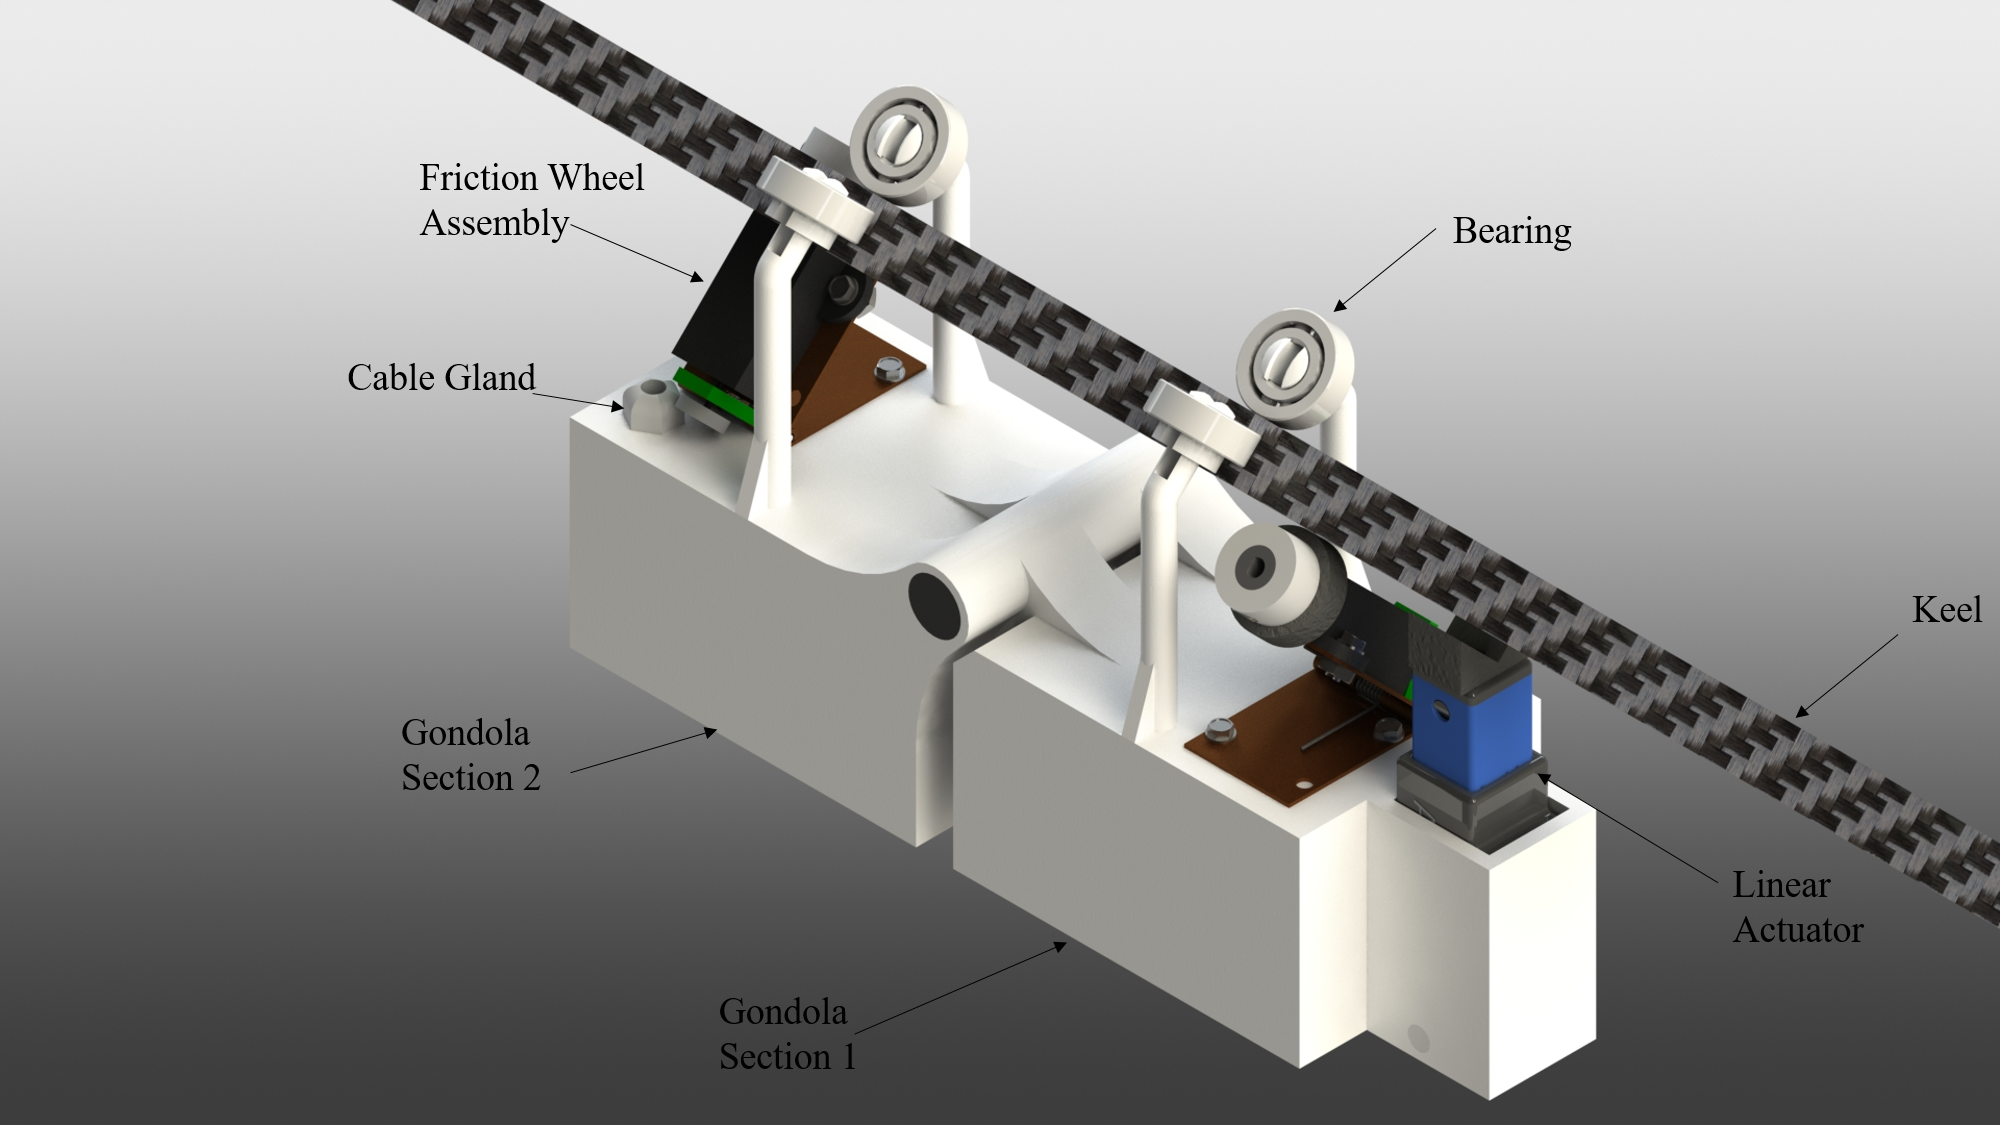
\includegraphics[width=.8\linewidth]{img/design/gondola/gondolaIsometric.png}
	\caption{Isometric View of the Gondola Assembly on the Keel}
	\label{fig:gondolaIsomeric}
\end{figure}

\begin{figure}[H]
	\centering
	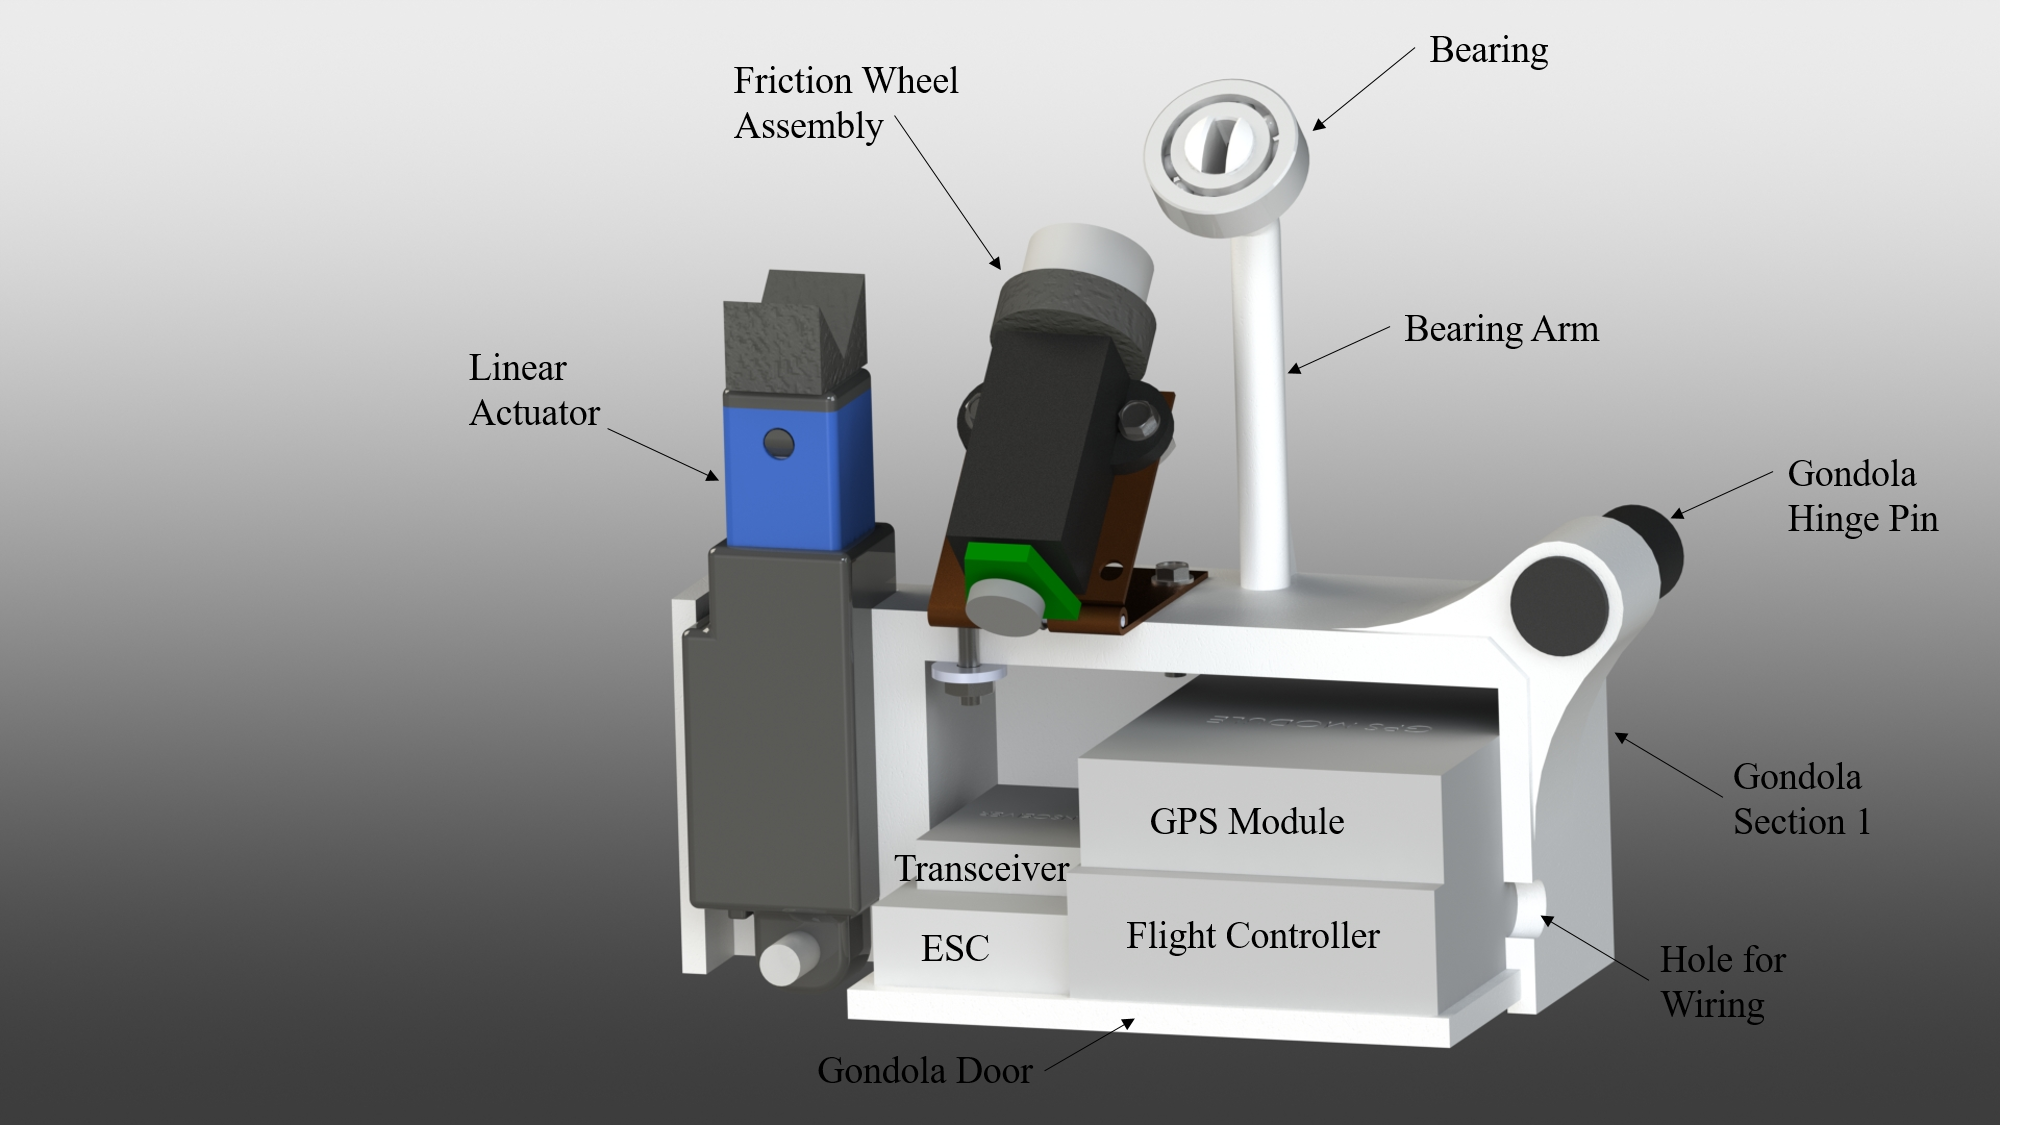
\includegraphics[width=.8\linewidth]{img/design/gondola/gondolaPartialSection.png}
	\caption{Partial Section of Gondola 1 (Components)}
	\label{fig:gondolaPartialSection}
\end{figure}

\begin{figure}[H]
	\centering
	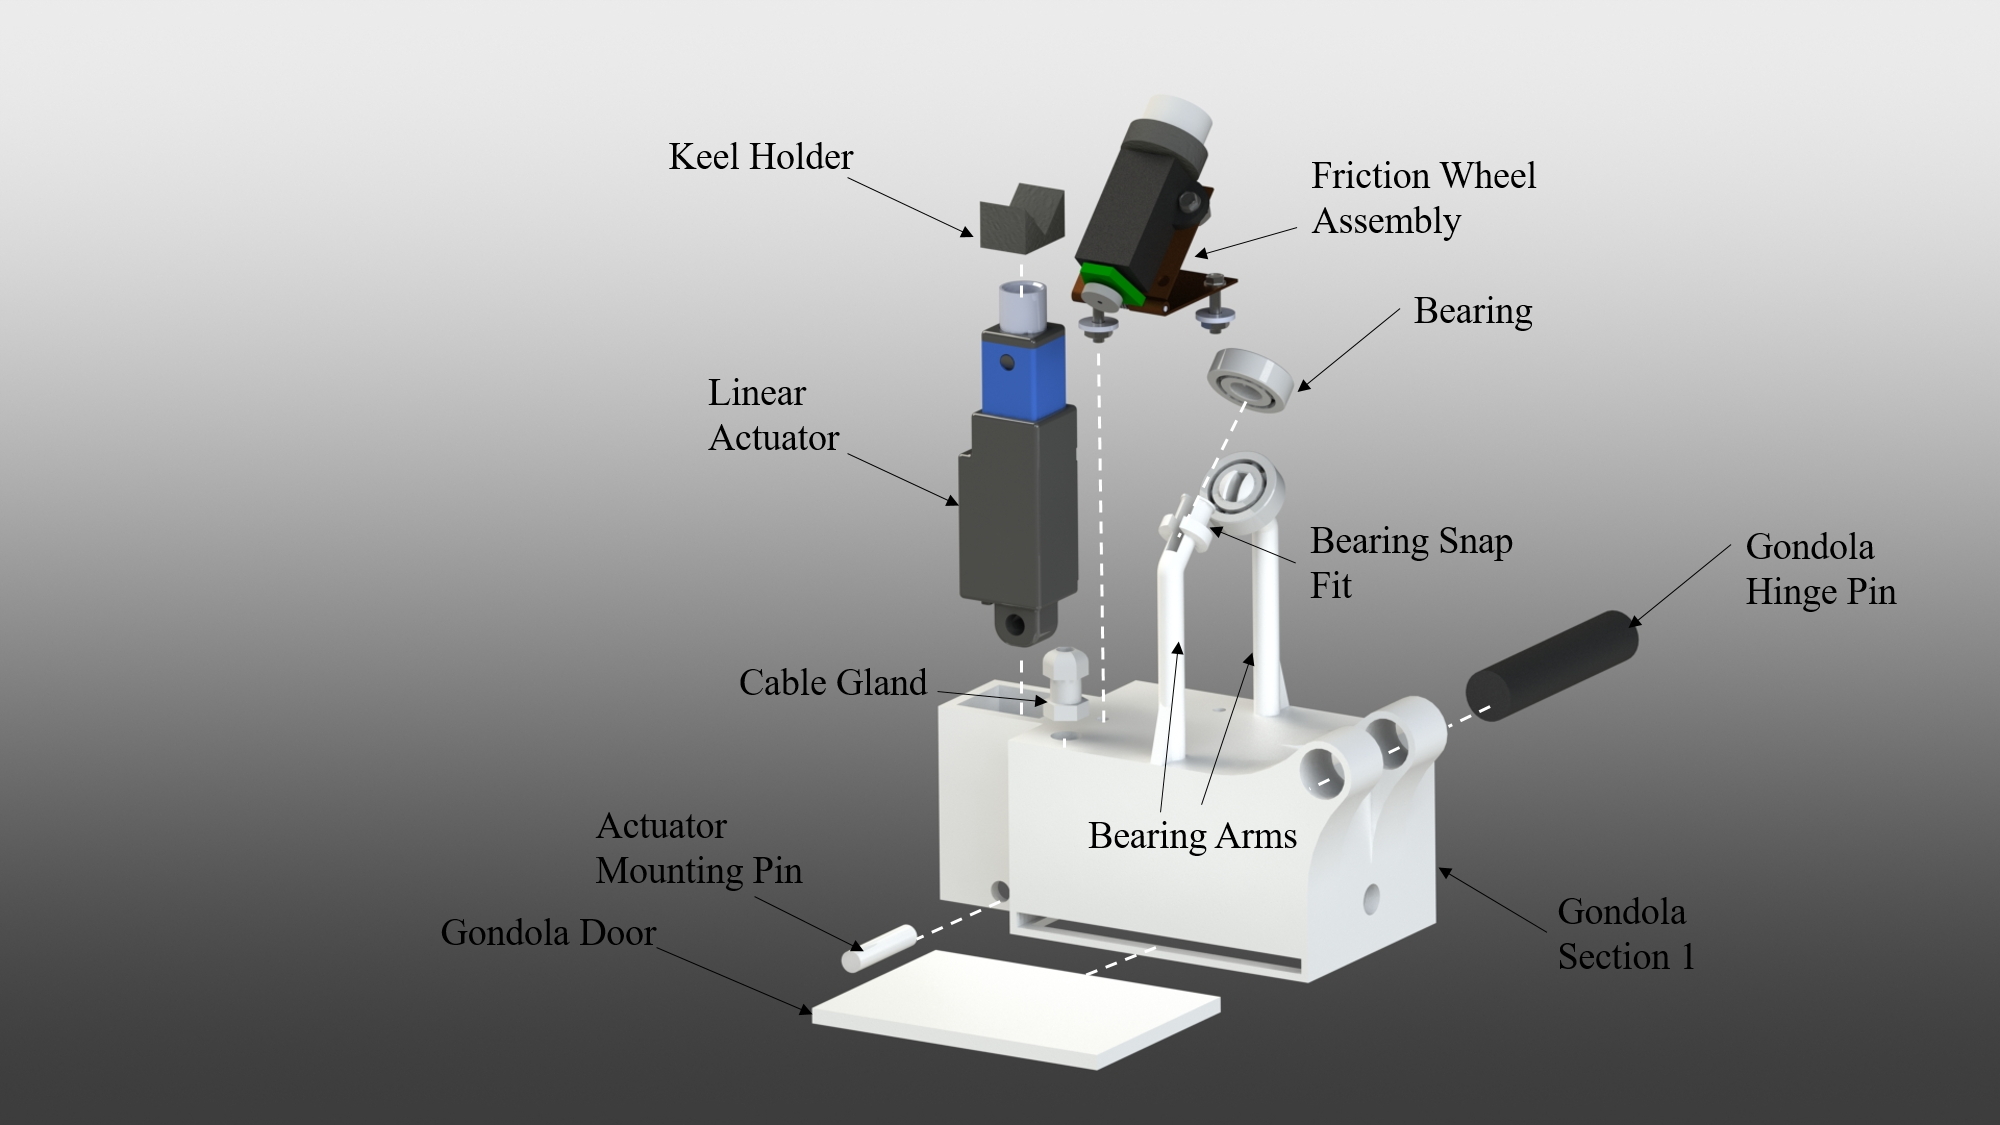
\includegraphics[width=.8\linewidth]{img/design/gondola/gondola1ExplodedView.png}
	\caption{Gondola 1 Exploded View}
	\label{fig:gondola1ExplodedView}
\end{figure}

\begin{figure}[H]
	\centering
	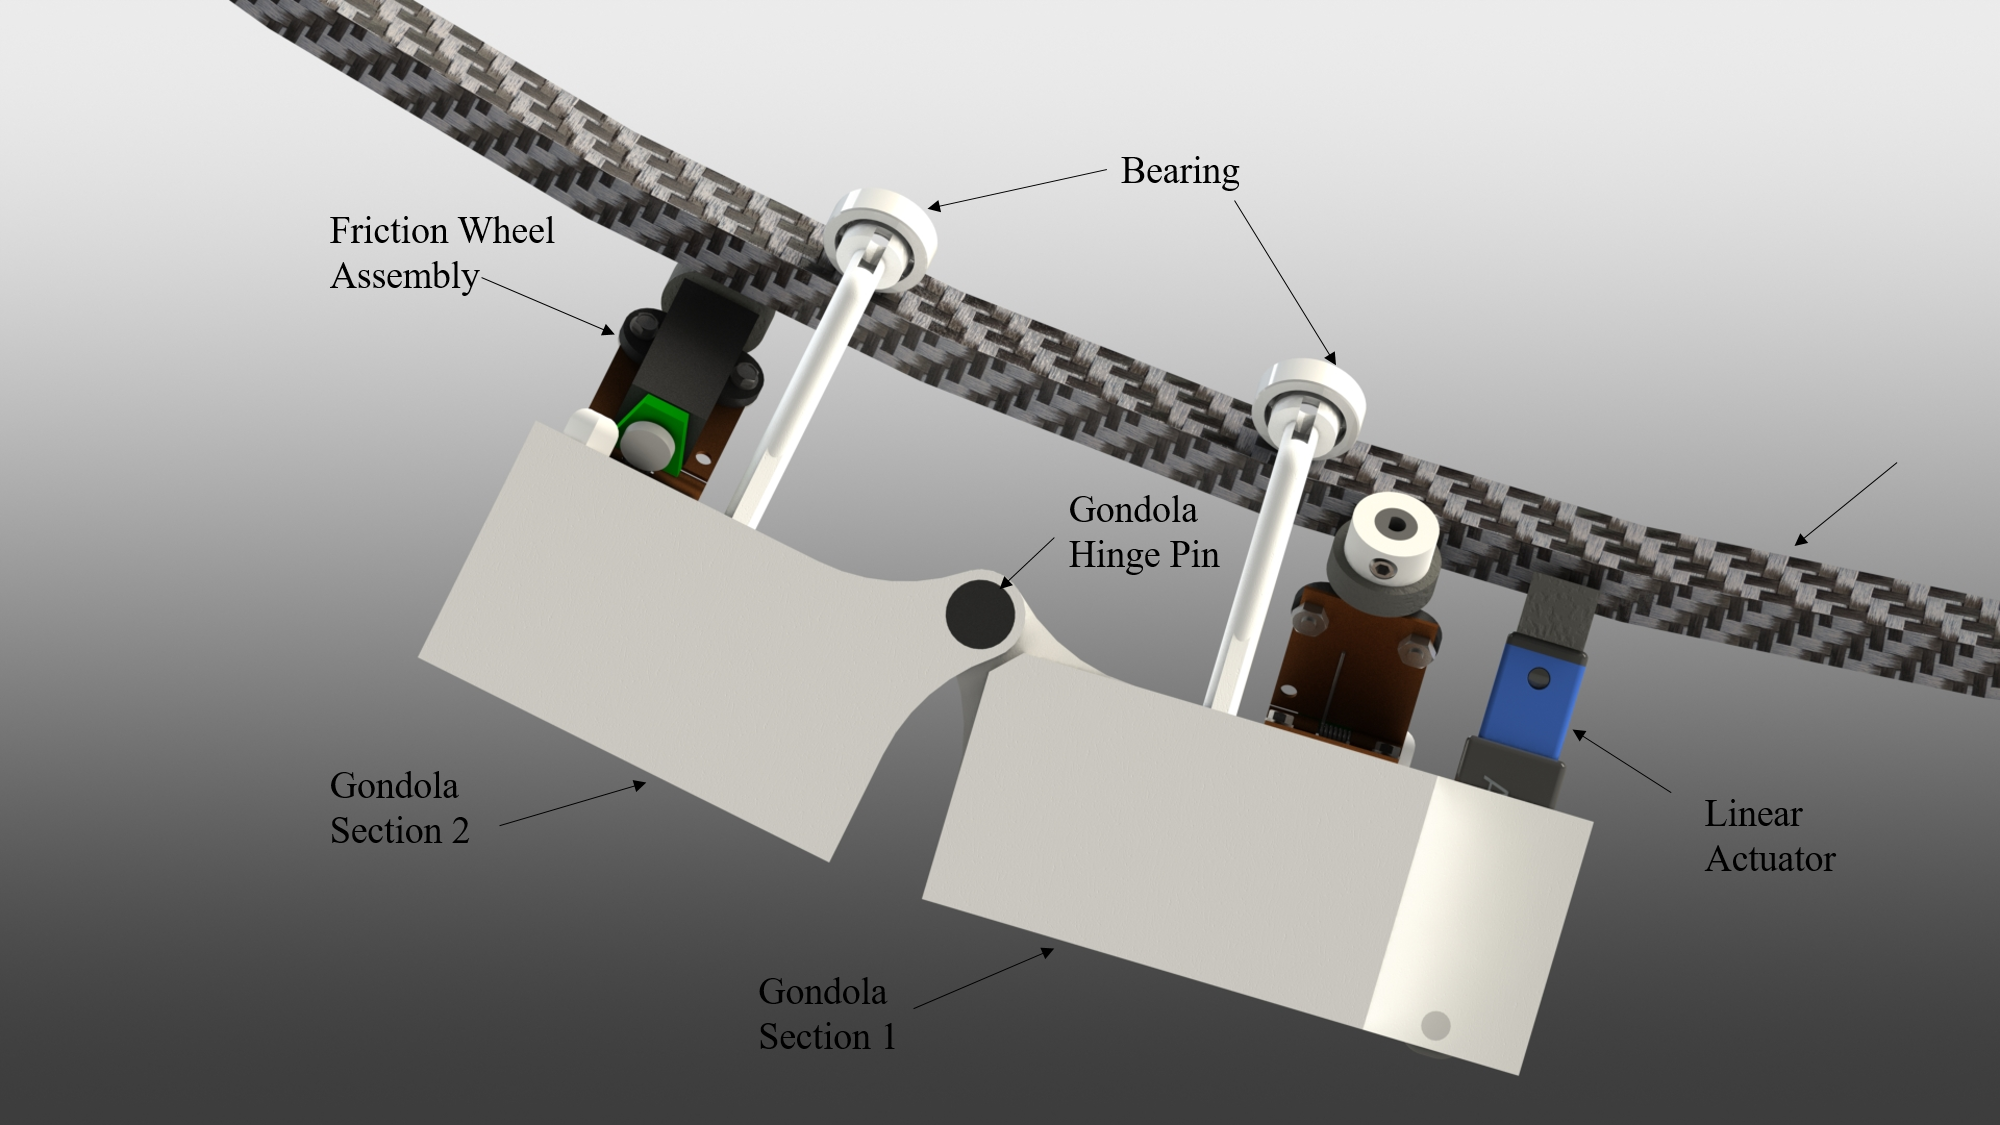
\includegraphics[width=.8\linewidth]{img/design/gondola/gondolaBent.png}
	\caption{Gondola Assembly on Curved Section of Keel}
	\label{fig:gondolaBent}
\end{figure}

\begin{figure}[H]
	\centering
	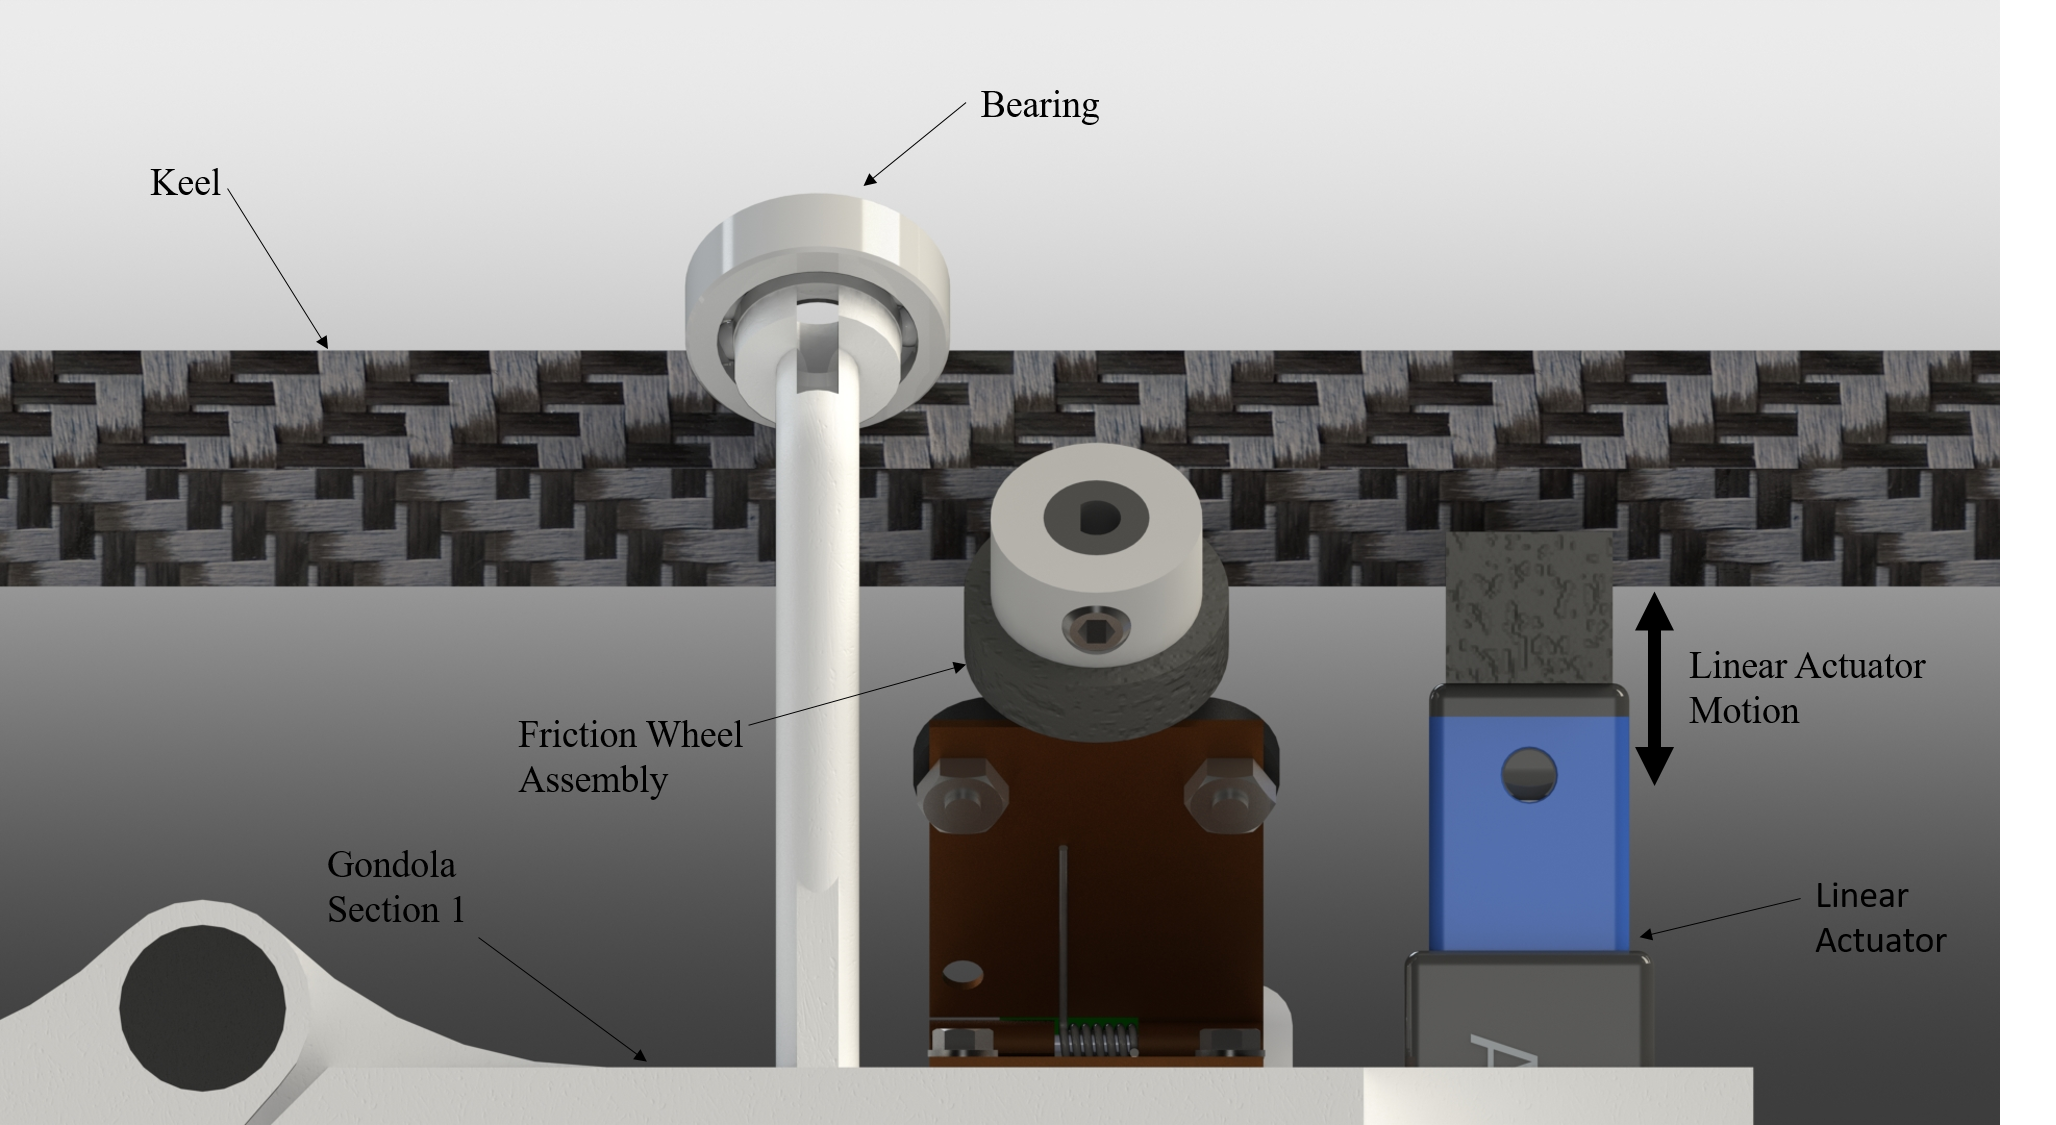
\includegraphics[width=.8\linewidth]{img/design/gondola/linearActuatorAndMotor.png}
	\caption{Linear Actuator Motion}
	\label{fig:linearActuatorAndMotor}
\end{figure}

\subsection{Friction Wheel}
The friction wheel must always be in contact with the keel, shown in Figure \ref{fig:frictionWheelOnGondola}. The friction wheel is made from 55D rubber, purchased off-the-shelf so it can deform when it is placed on the keel. A shaft adapter is necessary to bridge the gap between the motor shaft and the friction wheel, as the two sizes are not compatible. The shaft adapter will be 3D printed, and held in place by an existing set screw in the friction wheel. To ensure adequate pressure on the keel, the friction wheel assembly is mounted on a hinged bracket equipped with a torsion spring at the pin, as seen in Figure \ref{fig:explodedFrictionWheel}. The motor used can rotate in both directions, making it useful as a brake also. A magnetic encoder allows for accurate positioning of the gondola sections, independently allowing for redundancy between the two motors. The motor is mounted to the bracket using two nuts and two bolts. The bracket is mounted to the gondola using 2 nuts, 2 bolts and 2 washers. The bracket and hinge will be manufactured in house with a sourced torsion spring.
\\
\begin{figure}[H]
	\centering
	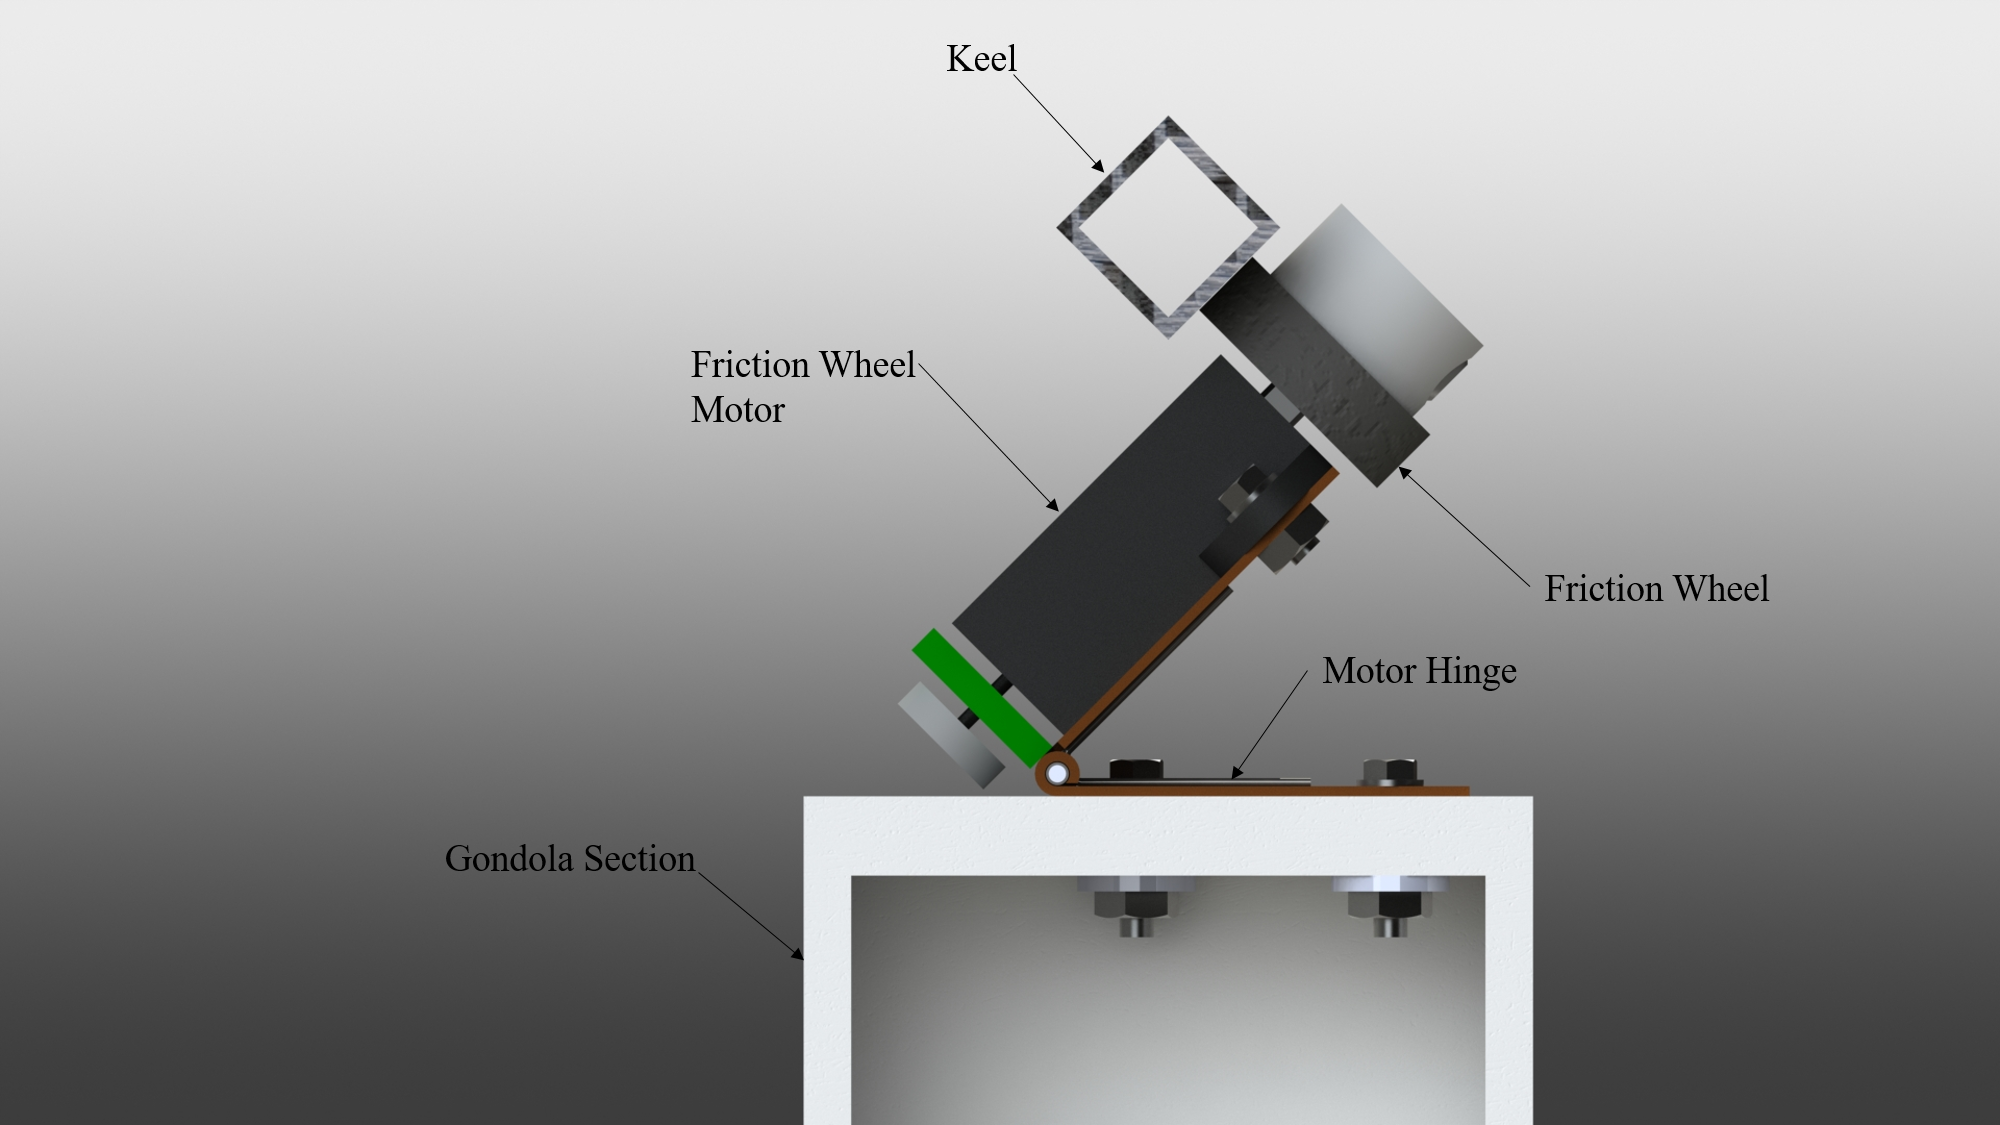
\includegraphics[width=.8\linewidth]{img/design/gondola/frictionWheelOnGondola.png}
	\caption{Friction Wheel Interfacing with the Keel}
		\label{fig:frictionWheelOnGondola}
\end{figure}
\begin{figure}[H]
	\centering
	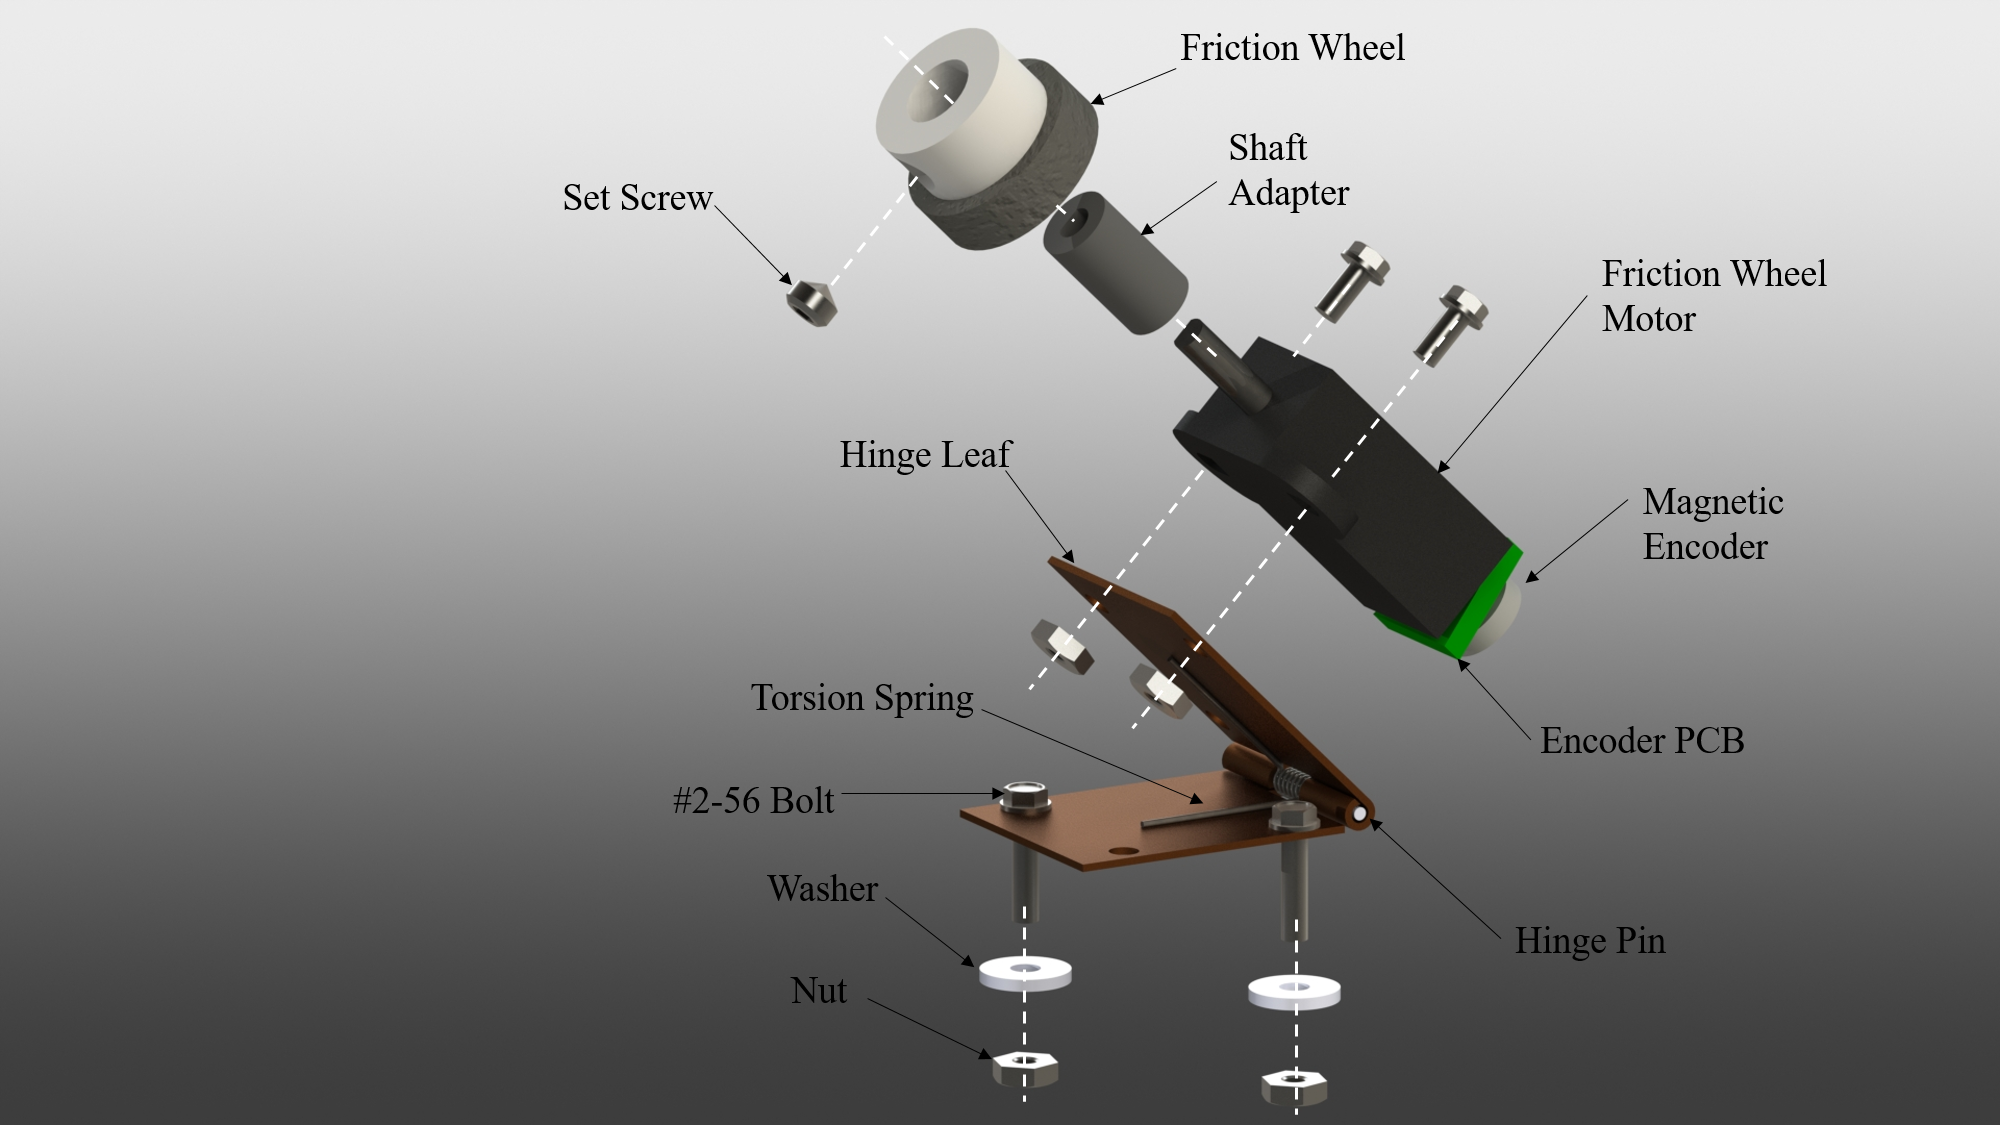
\includegraphics[width=.8\linewidth]{img/design/gondola/explodedFrictionWheel.png}
	\caption{Exploded View of the Friction Assembly}
	\label{fig:explodedFrictionWheel}
\end{figure}
\subsection{Bearings}
Bearings are placed on top of the keel to support the weight of the gondola and counter the force applied to the keel by the friction wheel. The bearings act as wheels turning and slipping along the keel. Low weight, plastic bearings will be used. The bearings are mounted using a snap fit design, that can be seen in \ref{fig:gondola1ExplodedView}, where the bearing is held in place by a diameter slightly larger than its own. The bearing is placed over the piece, deflecting it until the bearing can slip past the overhang where the snap fit piece elastically snaps back into its original position, securely holding the bearing.
\\
\subsection{Linear Actuator}
A linear actuator is housed on one of the two sections of the gondola. The linear actuator is to be activated when the gondola is not moving to hold its position on the keel. The motion can be seen in Figure \ref{fig:linearActuatorAndMotor} A custom 3D printed piece is outfitted to the top of the actuator (Keel Holder) in a V-shape to mesh ideally with the keel, as seen in Figure \ref{fig:gondola1ExplodedView}. The V-shaped 3D printed surface will then be coated with a Plasti Dip${\textregistered}$ like coating, to reduce the likelihood of tearing the polyurethane cover on the keel.  The  linear actuator chosen has a holding force of 45N without constant power, making it ideal for run time. It is also water resistant to the IP54 standard. 
\\
\subsection{Door and Components}
The gondola features a sliding door (the motion can be seen in Figure \ref{fig:gondola1ExplodedView}), to ease the process of component charging and changing. The door relies upon an interference fit to stay in place and components are placed on top of the door once it is half closed. See Figure \ref{fig:gondolaPartialSection} (selective cross-section). The door will be 3D printed also.
\\
\section{Keel}
Figure \ref{fig:keelAssemblyCompressedThruster} shows the keel assembly in a condensed form. The two straight and one curved sections of the keel and the envelope support originate from Dr. Lanteigne's design. Sections of the keel are joined using connectors that rely on interference fits, also designed by Dr. Lanteigne, but modified and machined for better material properties. The envelope support slides into a slot on the keel connectors remaining in position by bottoming out. The surface will also be lathered with epoxy to prevent the piece from falling out when the airship is perpendicular to the ground. Thrusters are mounted on carbon fibre arms that also slide into the connector, maintaining position by bottoming out as well. The section shown in Figure \ref{fig:thrusterArmConnectorCrossSection} displays the bottoming out and Figure \ref{fig:thrusterArmConnectorPiece} shows the fit. 3D printed end stops are inserted in either end of the keel using an interference fit identical to the connectors. The end stop design can be seen in Figure \ref{fig:keelEndCap}. These stops are slightly larger than the size of the keel, effectively interfering with the gondola wheels, keeping it from rolling off the ends of the keel. All geometries in the keel assembly are fixed in relation to the airship with the exception of the thrusters.
\\
\begin{figure}[H]
	\centering
	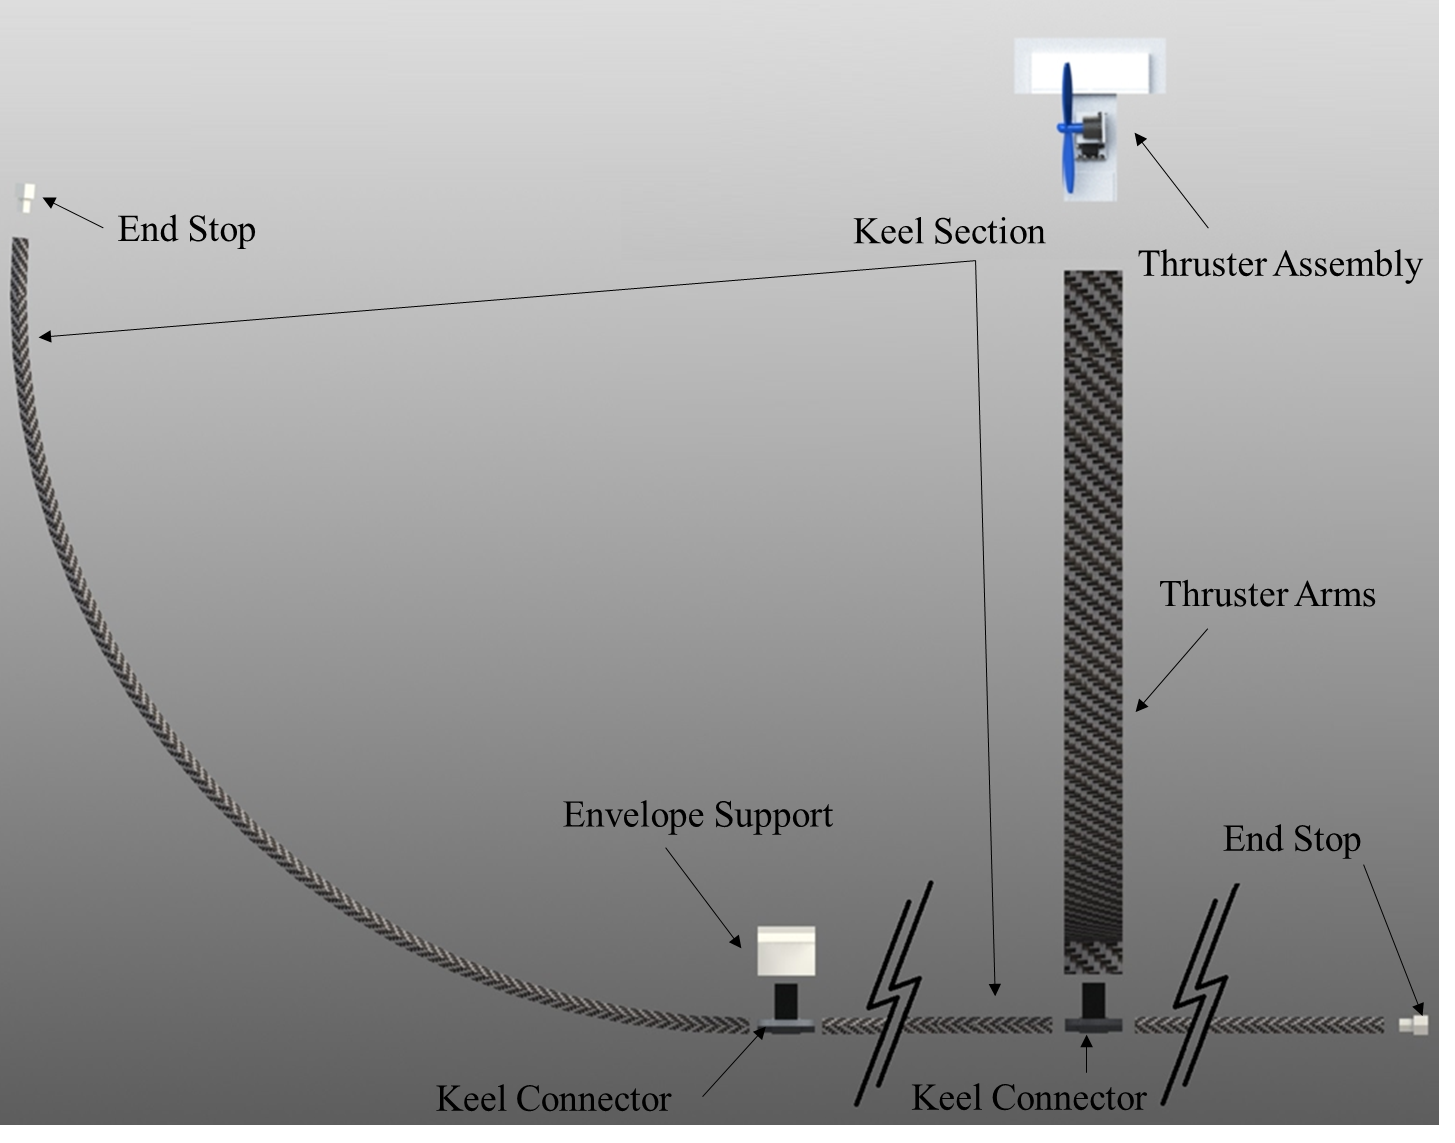
\includegraphics[width=.8\linewidth]{img/design/keel/keelAssemblyCompressedThruster.png}
	\caption{Overall Keel Assembly (Compressed)}
	\label{fig:keelAssemblyCompressedThruster}
\end{figure}
\begin{figure}[H]
	\centering
	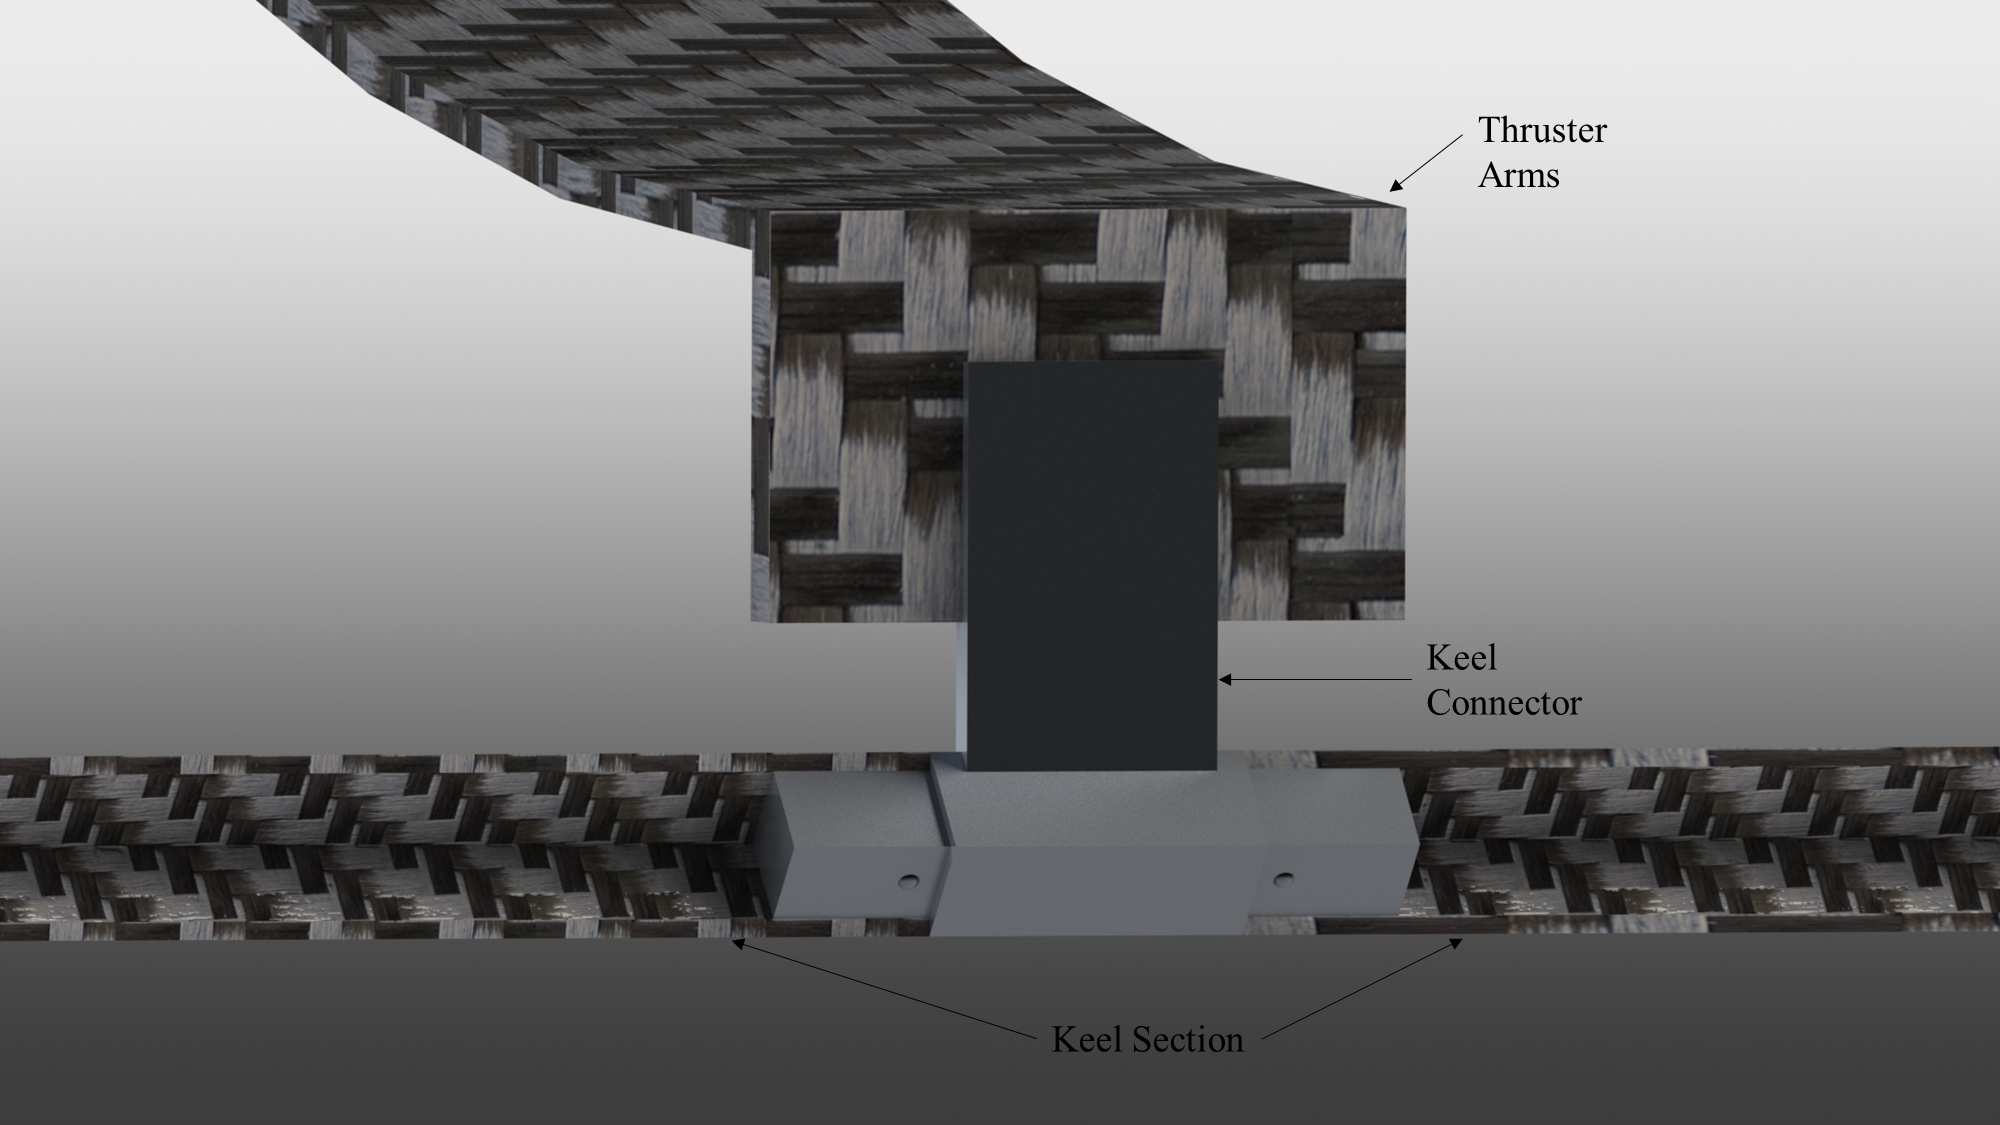
\includegraphics[width=.9\linewidth]{img/design/keel/thrusterArmConnectorCrossSection.png}
	\caption{Cross-Section of the Keel Connector}
	\label{fig:thrusterArmConnectorCrossSection}
\end{figure}
\begin{figure}[H]
	\centering
	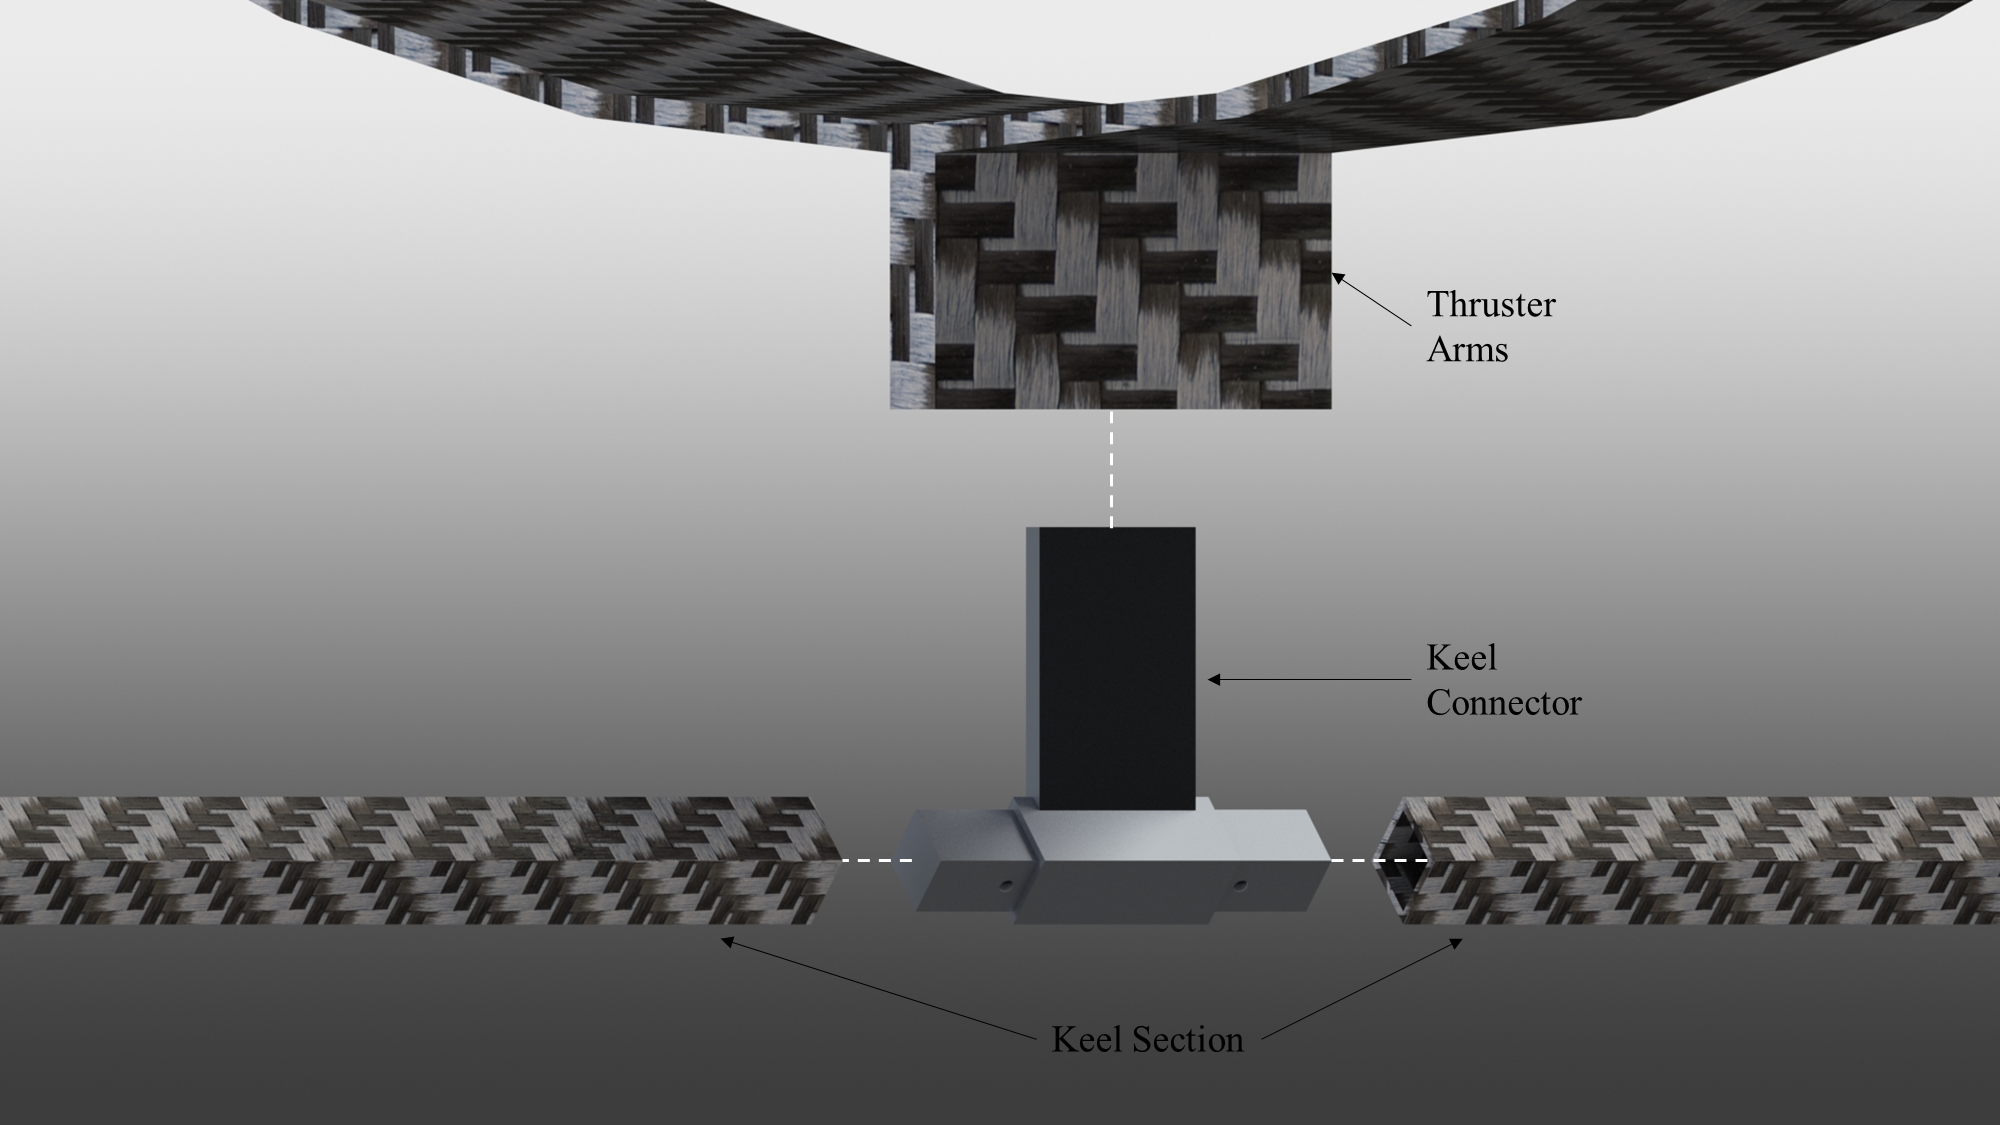
\includegraphics[width=.9\linewidth]{img/design/keel/thrusterArmConnectorPiece.png}
	\caption{Connector Piece Assembling}
	\label{fig:fig:thrusterArmConnectorPiece}
\end{figure}
\begin{figure}[H]
	\centering
	\includegraphics[width=.8\linewidth]{img/design/keel/keelEndCap.png}
	\caption{Keel End Stop}
	\label{fig:keelEndCap}
\end{figure}


\subsection{Thrusters}
The thruster arms are made from carbon fibre that will be made in house by laying sheets of carbon fibre on a balloon mold. A CNC machined aluminum plate is attached to the U-shaped carbon fibre arms by welding a machined cap piece onto the plate, then inserting the carbon fibre arm into it and applying epoxy. The aluminum plate and bearing arms are built in a way that will interfere with the airship, causing compression of the helium and polyurethane sheet. This will enable contact between the airship and plate, increasing the surface area for the double sided tape union. This mounting technique can be seen in Figure \ref{fig:thrusterOnKeel} The full assembly can be seen in Figure \ref{fig:thrusterAssembly}.  Components are housed inside a 3D printed casing that features a 3D printed door, similar to the gondola. Figure \ref{fig:plateAssembly} displays how the components are mounted on the plate. The components for each thruster include, a receiver, a battery and a BESC. The components are located above the centre of volume of the airship in the z-direction, raising the centre of mass. These components are well covered from the rain and any splashing water. With the casing above the servo motor, the servo motor is shielded from rain in normal flying conditions.\\
\begin{figure}[H]
	\centering
	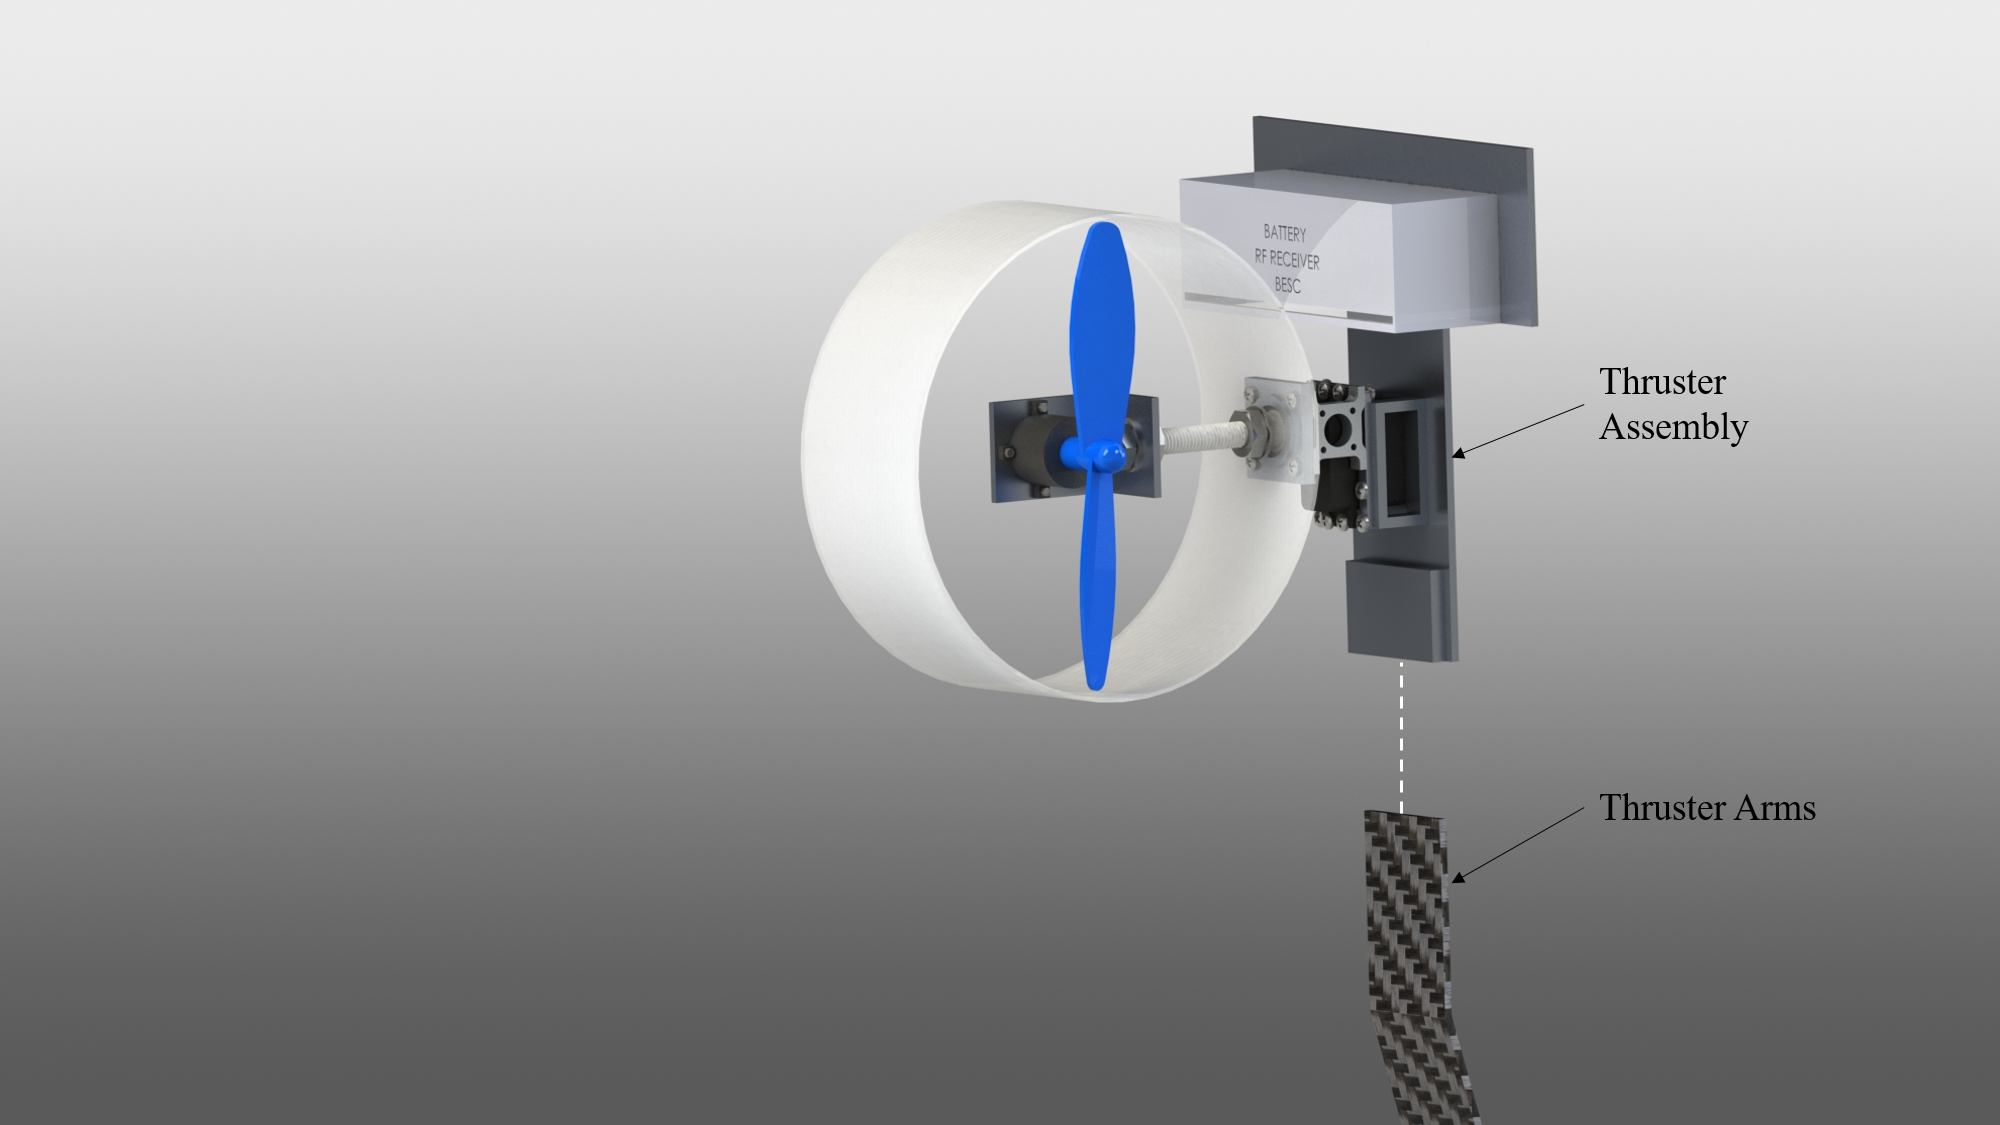
\includegraphics[width=.8\linewidth]{img/design/thruster/thrusterOnKeel.png}
	\caption{Thruster Assembly on Thruster Arm}
	\label{fig:thrusterOnKeel}
\end{figure}

\begin{figure}[H]
	\centering
	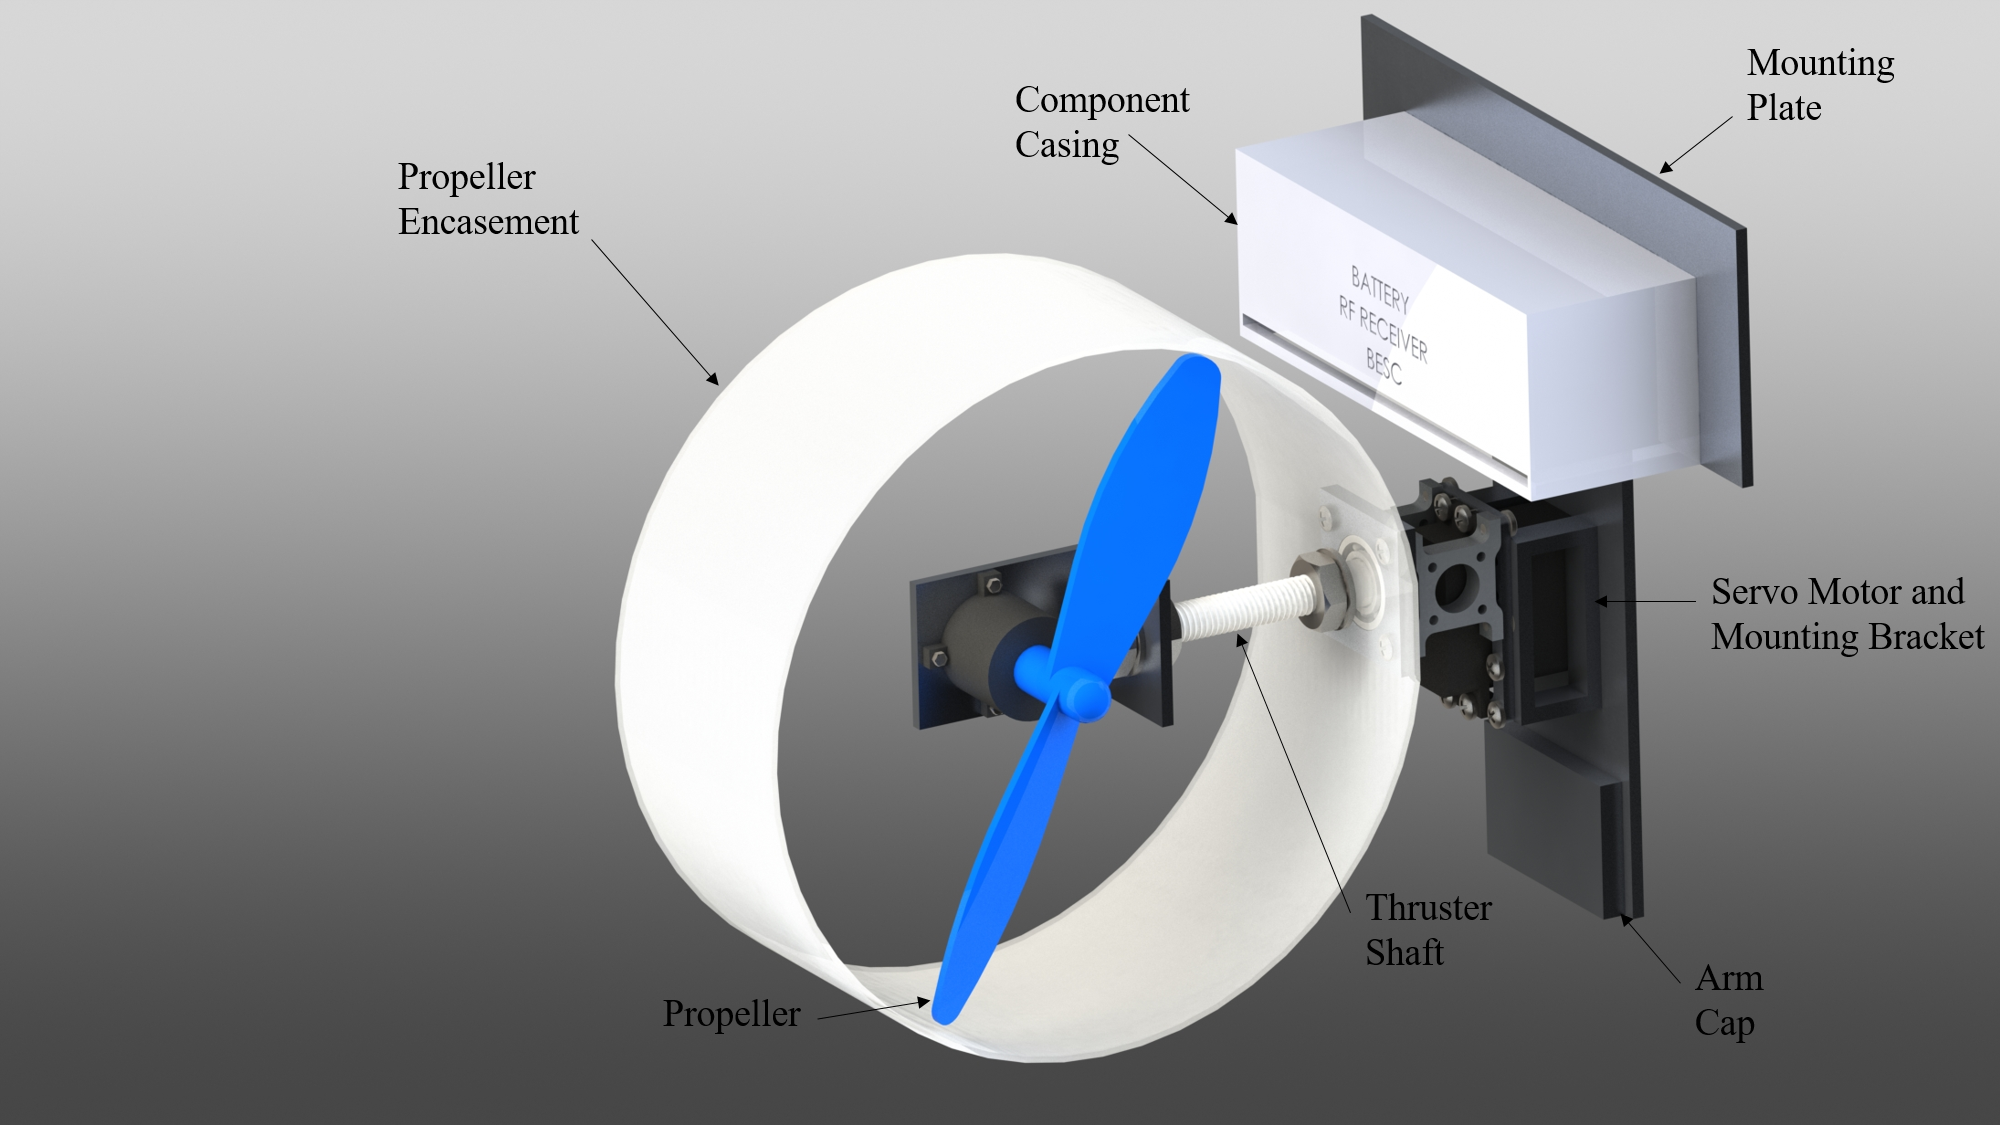
\includegraphics[width=.8\linewidth]{img/design/thruster/thrusterAssembly.png}
	\caption{Overall Thruster Assembly}
	\label{fig:thrusterAssembly}
\end{figure}

\begin{figure}[H]
	\centering
	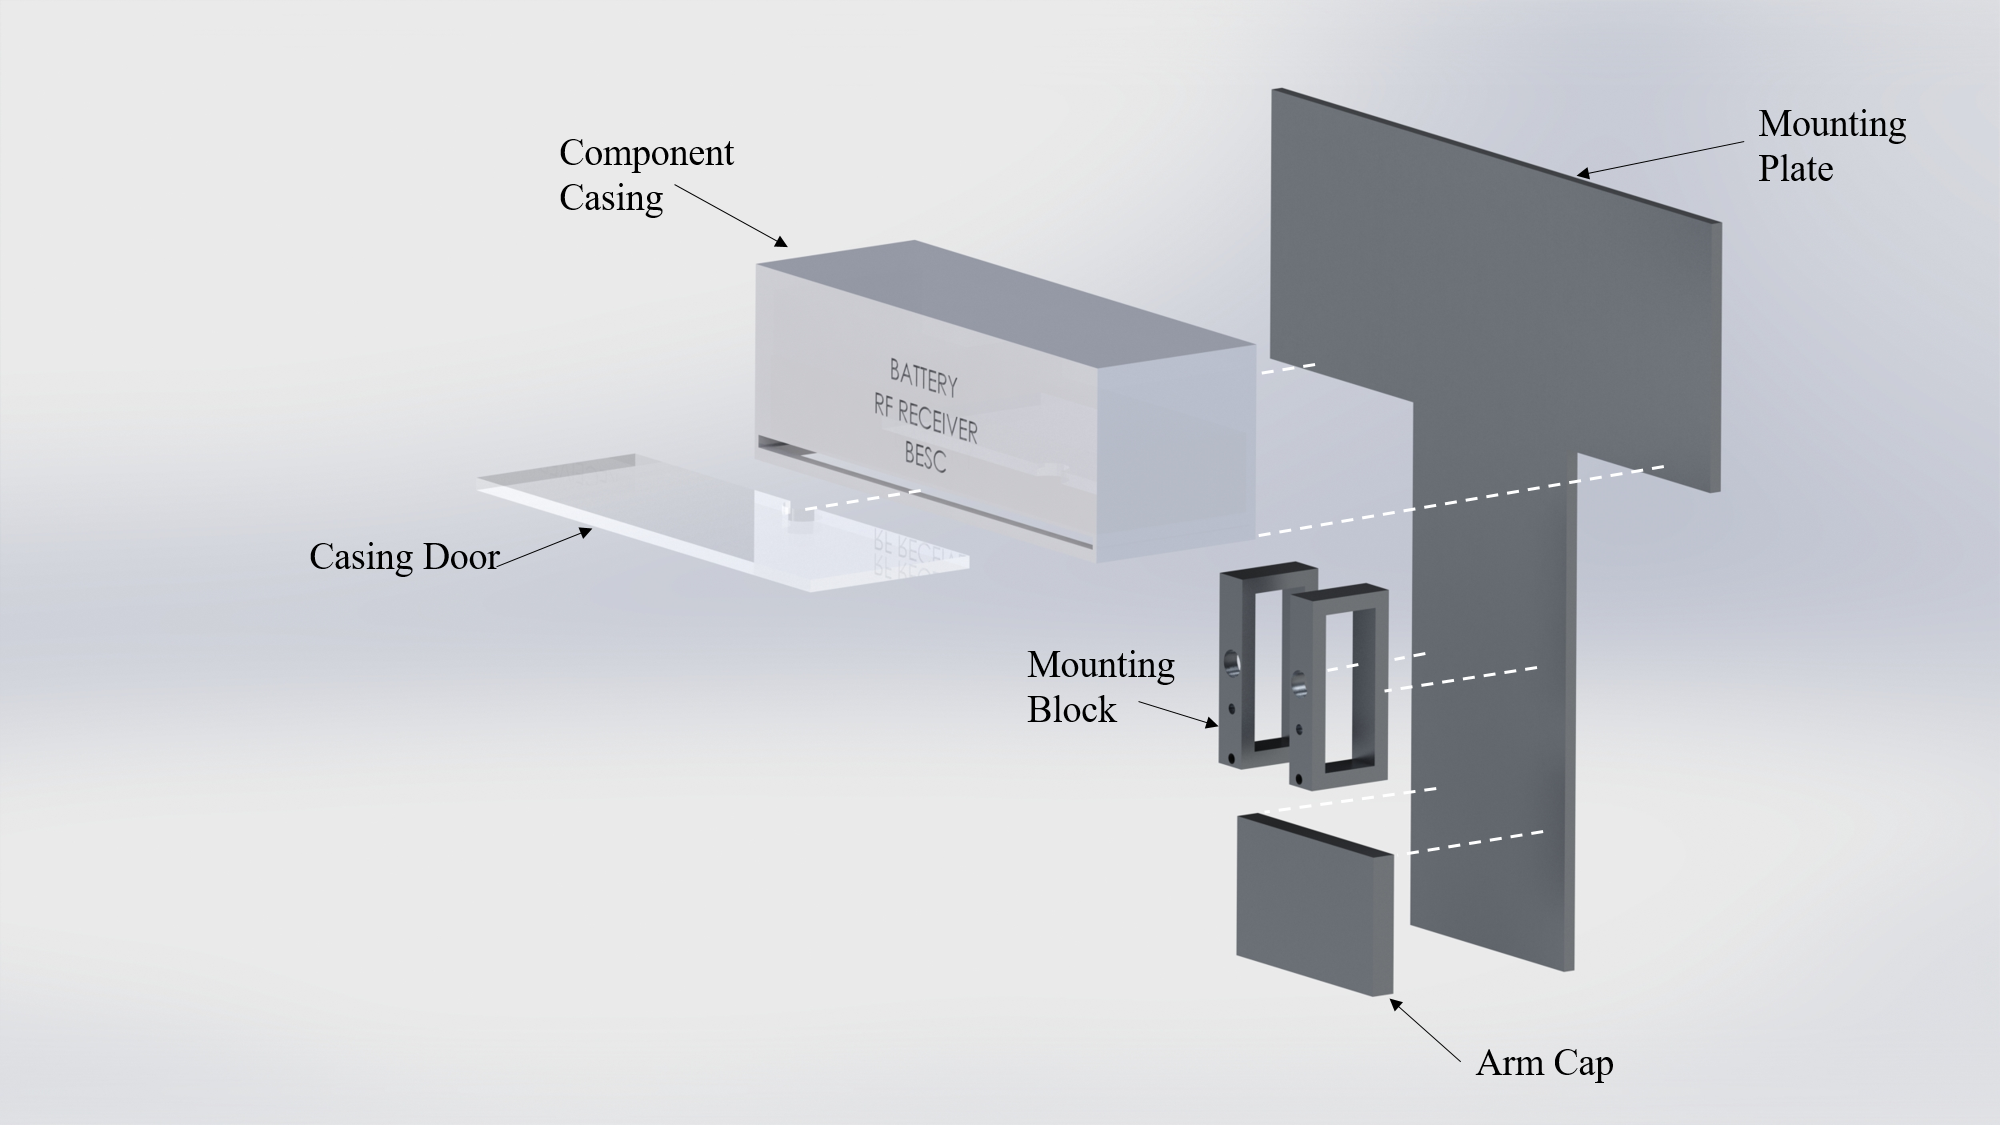
\includegraphics[width=.8\linewidth]{img/design/thruster/plateAssembly.png}
	\caption{Mounting Plate Exploded View}
	\label{fig:plateAssembly}
\end{figure}

 A servo motor is mounted to the plate using aluminum blocks along with off-the-shelf assembly, as seen in Figure \ref{servoAssembly}. A bearing and custom machined bracket are added to the off-the-shelf to support the shaft attached to the servo motor. Figure \ref{fig:shaftAssembly} shows the bearing bracket, bearing and shaft. The custom machined bracket features a shoulder to enable the shaft to support minimal and unexpected axial loads as well as to ease in the pressing of the bearing into the hub. figure ref{fig:??????????????????} shows the shoulder. The shaft will be machined to hollow, threaded on the outside and a shoulder that fits into the bearing inner race. The shaft is mounted to the spline on the servo, and an M3 screw is placed inside to shaft, axially fastening it to the servo, as the servo comes standard with a tapped hole. Several screws are used to securely fasten the servo to the supporting parts.
 \\
 
 \begin{figure}[H]
 	\centering
 	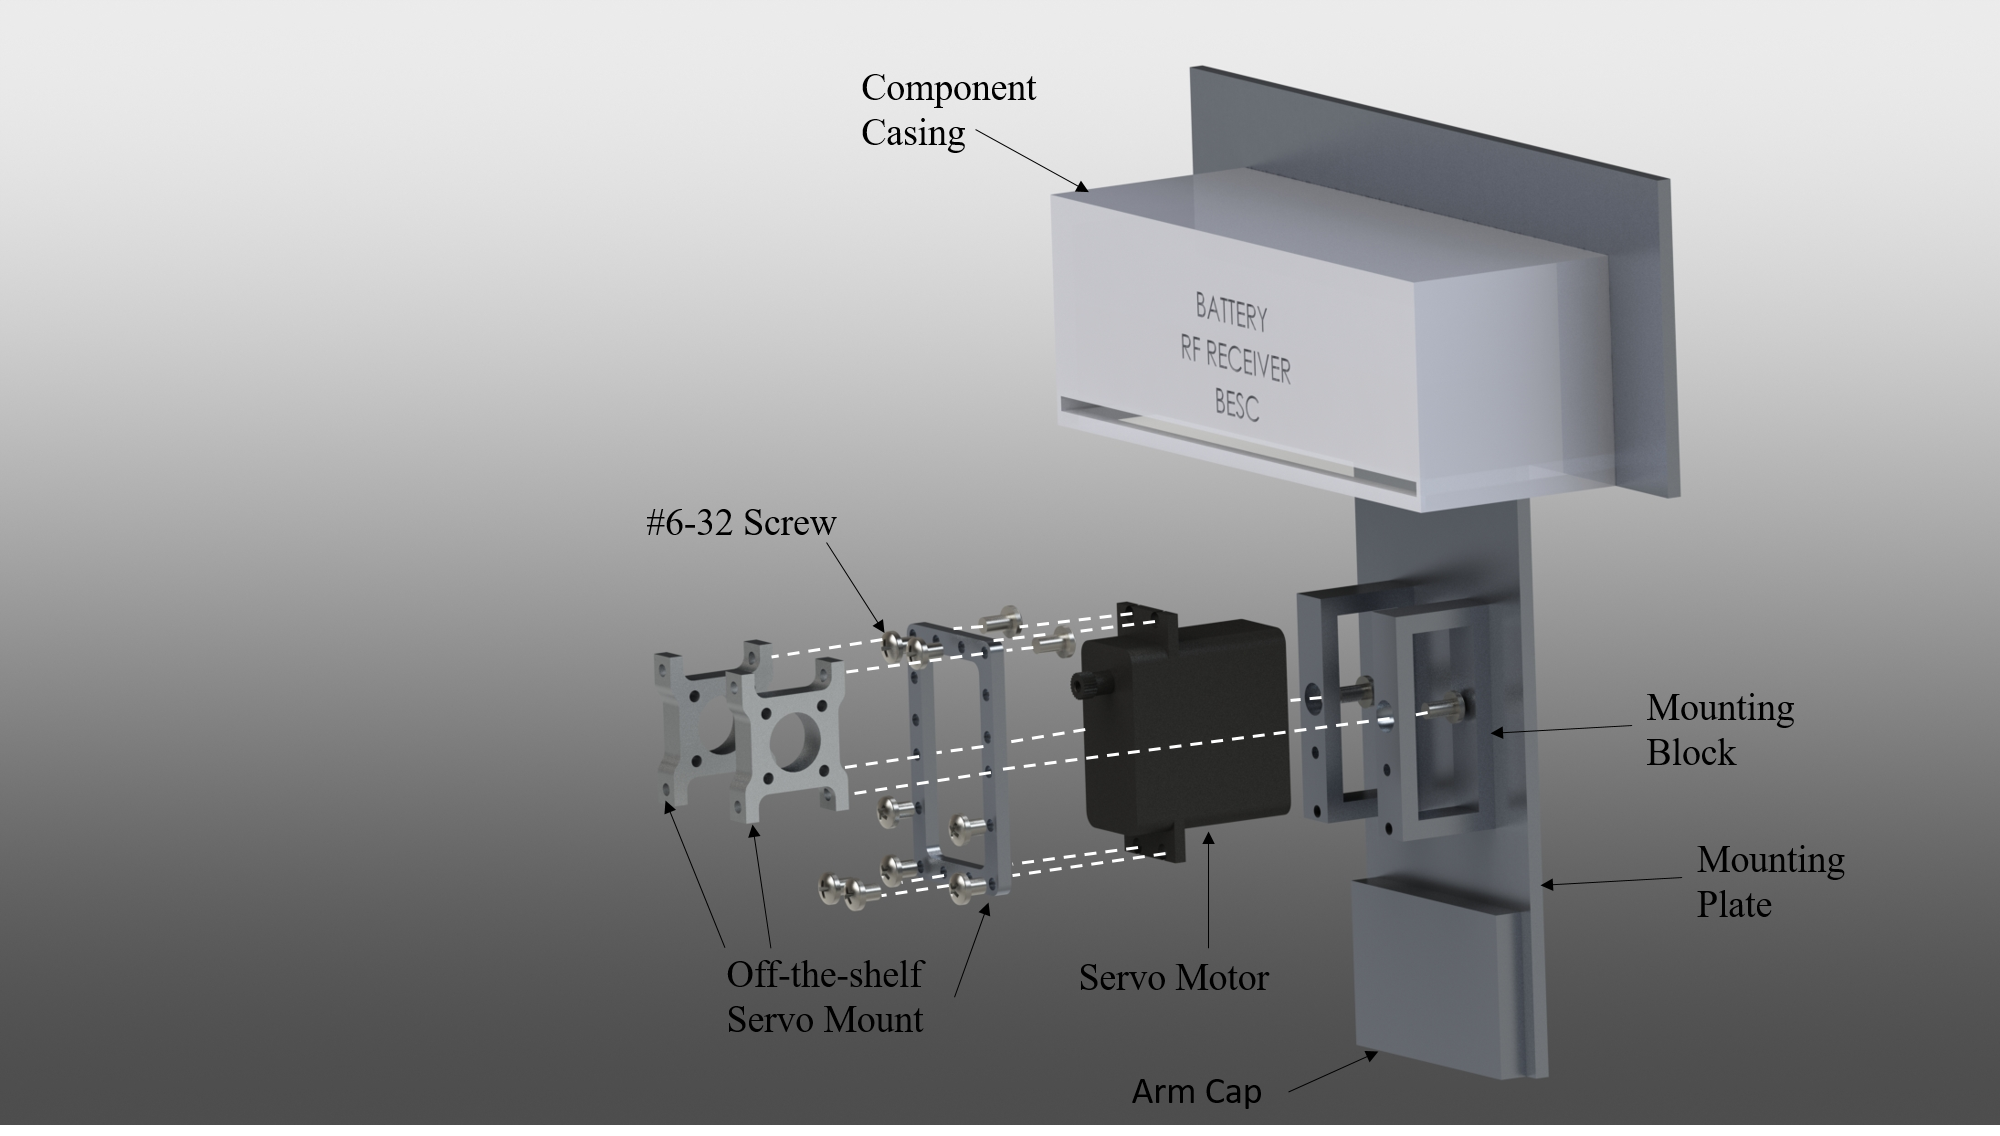
\includegraphics[width=.8\linewidth]{img/design/thruster/servoAssembly.png}
 	\caption{Servo Mounting Exploded View}
 	\label{fig:servoAssembly}
 \end{figure}
 
  \begin{figure}[H]
 	\centering
 	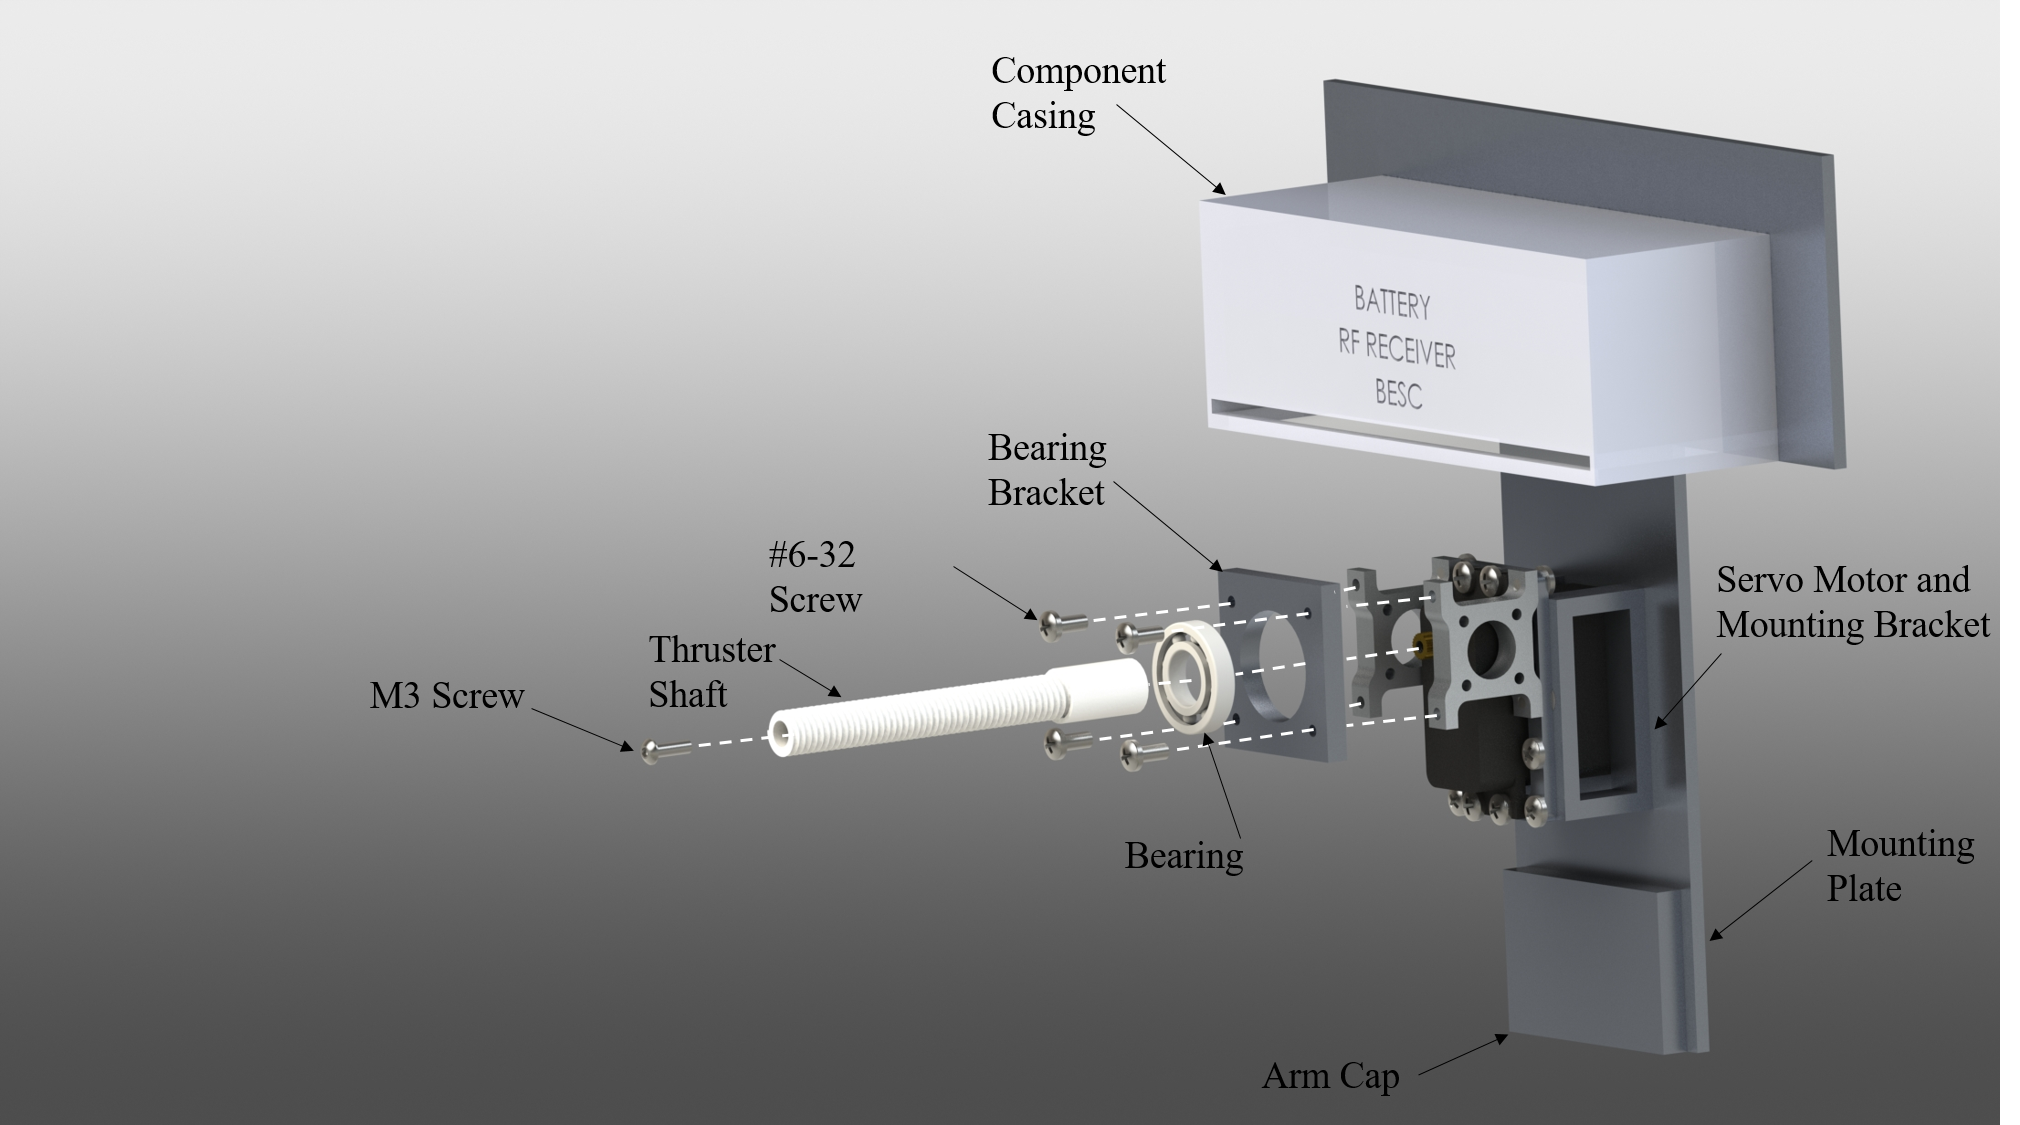
\includegraphics[width=.8\linewidth]{img/design/thruster/shaftAssembly.png}
 	\caption{Shaft Mounting Exploded View}
 	\label{fig:shaftAssembly}
 \end{figure}
 
The propeller motor is mounted on a machined propeller mounting bracket with tapped holes using screws, which is mounted on the shaft using washers and nuts. Figures \ref{fig:mountAssembly} and \ref{fig:propAssembly} show how the propeller and related parts will be mounted. The propeller is mounted to the motor using a standard interference fit, given that these are both off-the-shelf parts. The propeller and motor are protected by a lightweight encasement (MANUFACTURED HOW????) that is mounted to the shaft by squeezing the plastic between a shoulder on the shaft and washer/nut combination. The encasement provides shielding of the propeller motor during forward flight conditions.\\

 \begin{figure}[H]
	\centering
	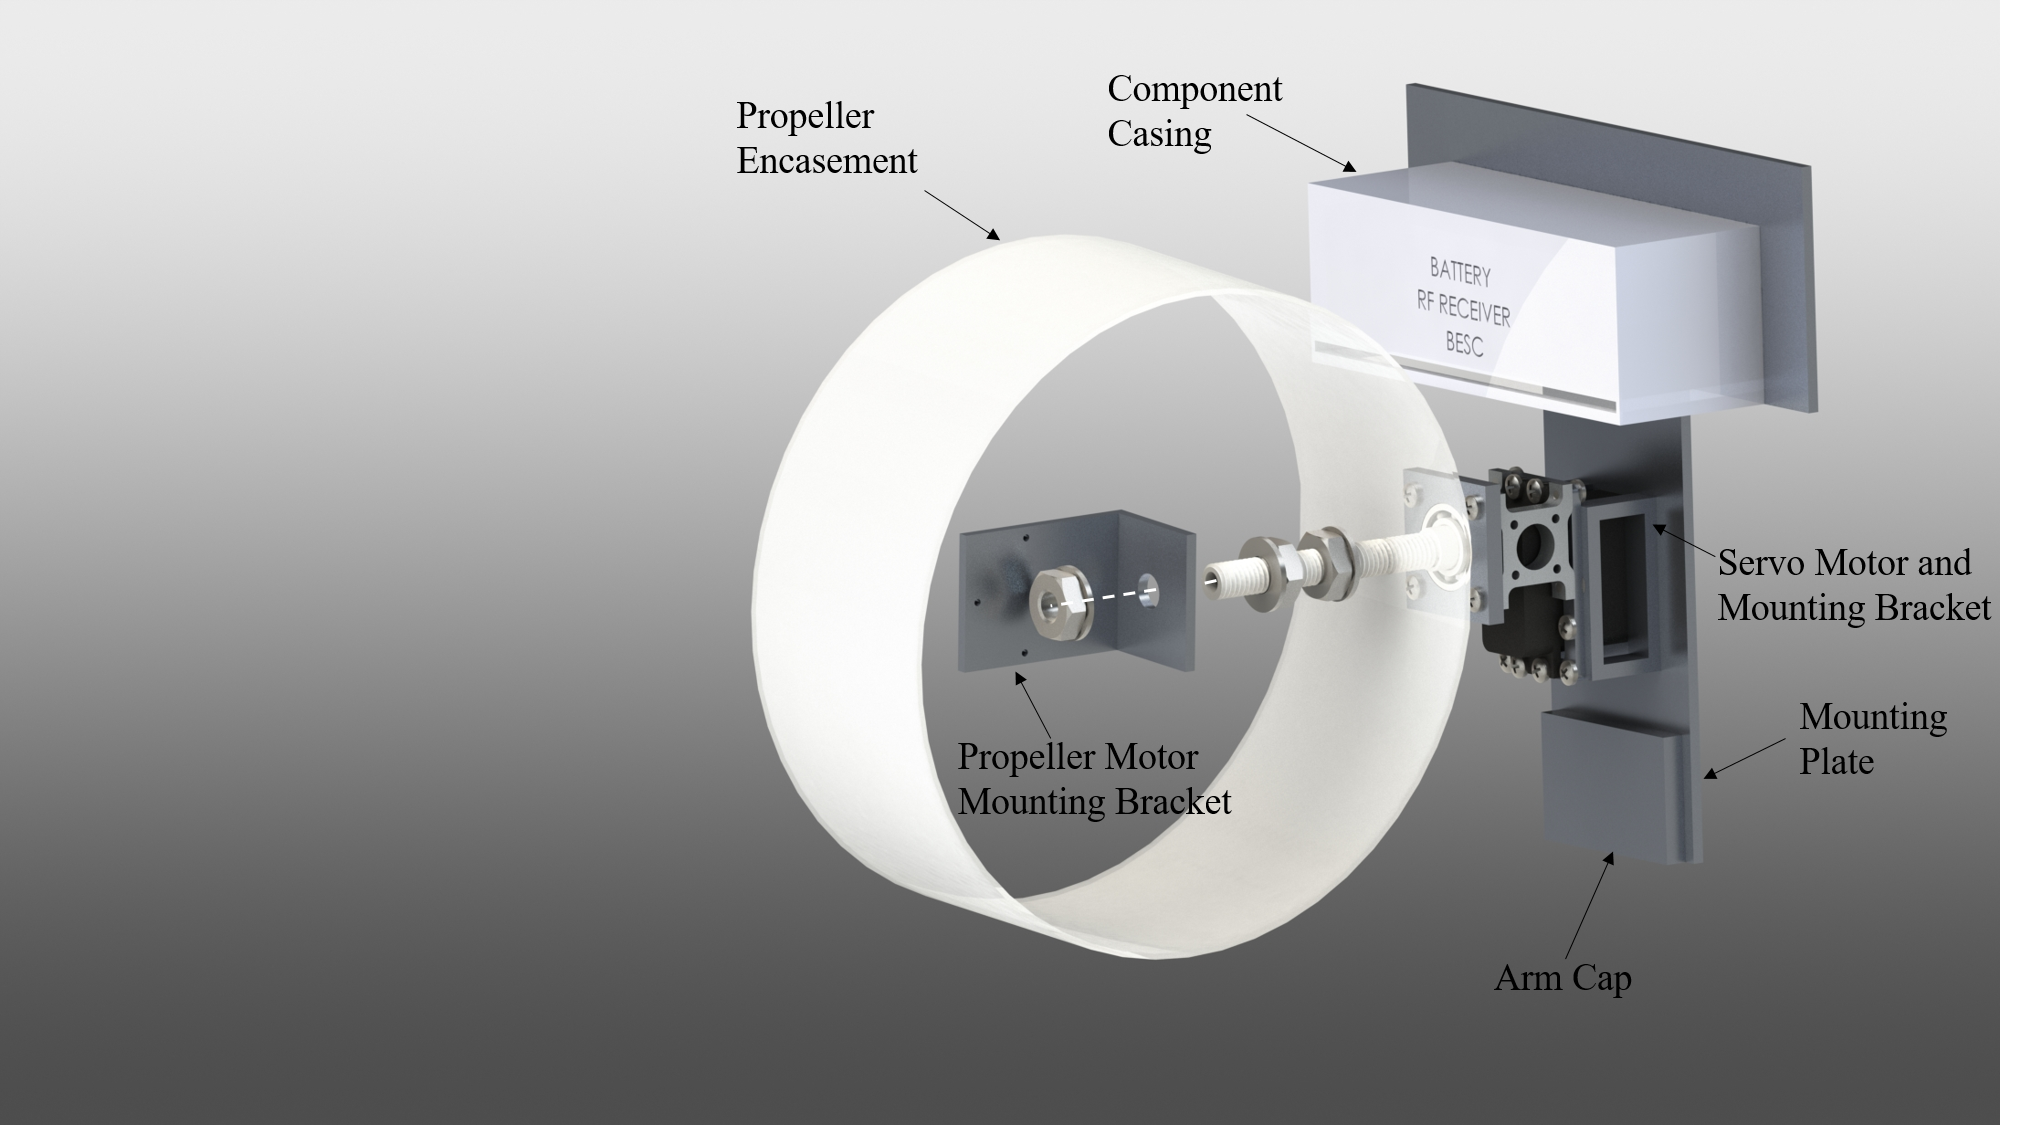
\includegraphics[width=.8\linewidth]{img/design/thruster/mountAssembly.png}
	\caption{Propeller Bracket Mounting Exploded View}
	\label{fig:mountAssembly}
\end{figure}

\begin{figure}[H]
	\centering
	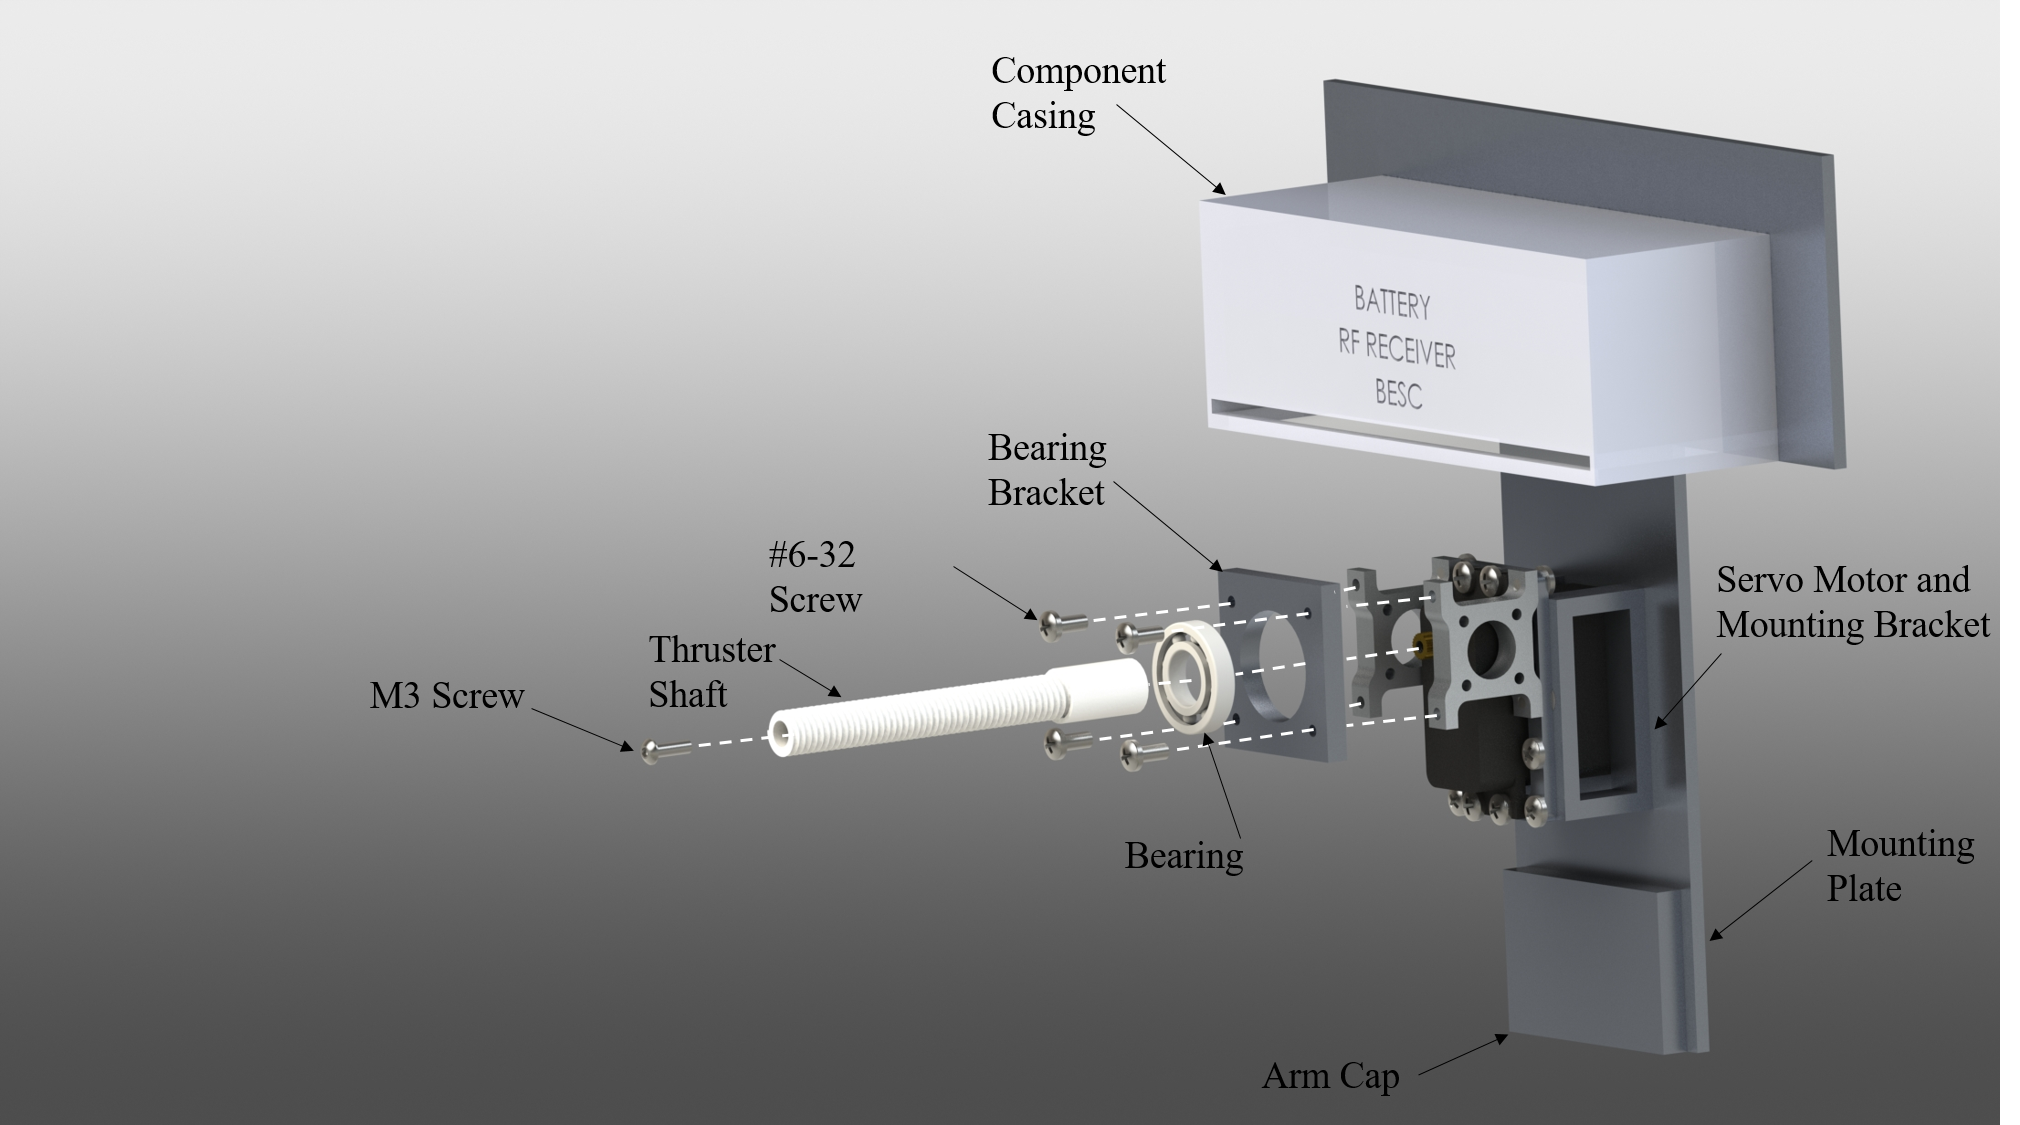
\includegraphics[width=.8\linewidth]{img/design/thruster/shaftAssembly.png}
	\caption{Propeller Exploded View}
	\label{fig:propAssembly}
\end{figure}

\section{Wiring}
Wiring for the airship is relatively straight forward as each motor assembly has an  independent power supply. Transmitters and receiver eliminate the need for wiring throughout the airship. Avoiding communication wiring significantly reduces the likelihood of wires tangling and causing jamming of parts. For the gondola, Figure \ref{fig:gondolaWiring} shows how wires will be routed. Components shown are rough dimensions taken from the specifications for each part, and include the start of the tails of the wires. Waterproofing is provided by cable glands for surfaces perpendicular to the fall of rain. Surfaces parallel to the fall of rain do not have waterproofing as these are not exposed to much water. The wires routed between the gondola will be provided with slack so the gondola can fold up to 10$^{\circ}$.
\\

\begin{figure}[H]
	\centering
	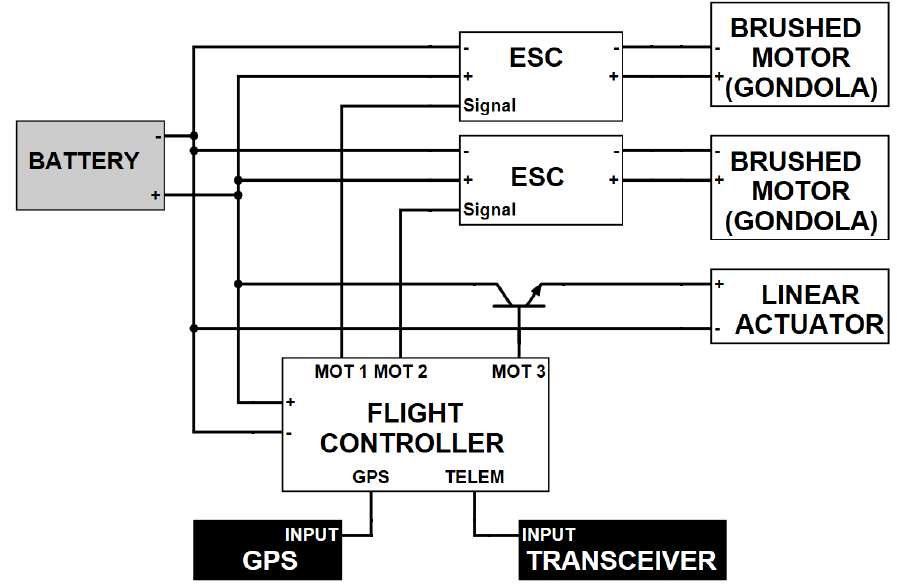
\includegraphics[width=.8\linewidth]{img/design/gondola/gondolaWiringSchematic.png}
	\caption{Gondola Component Wiring Schematic}
	\label{fig:gondolaWiringSchematic}
\end{figure}

\begin{figure}[H]
	\centering
	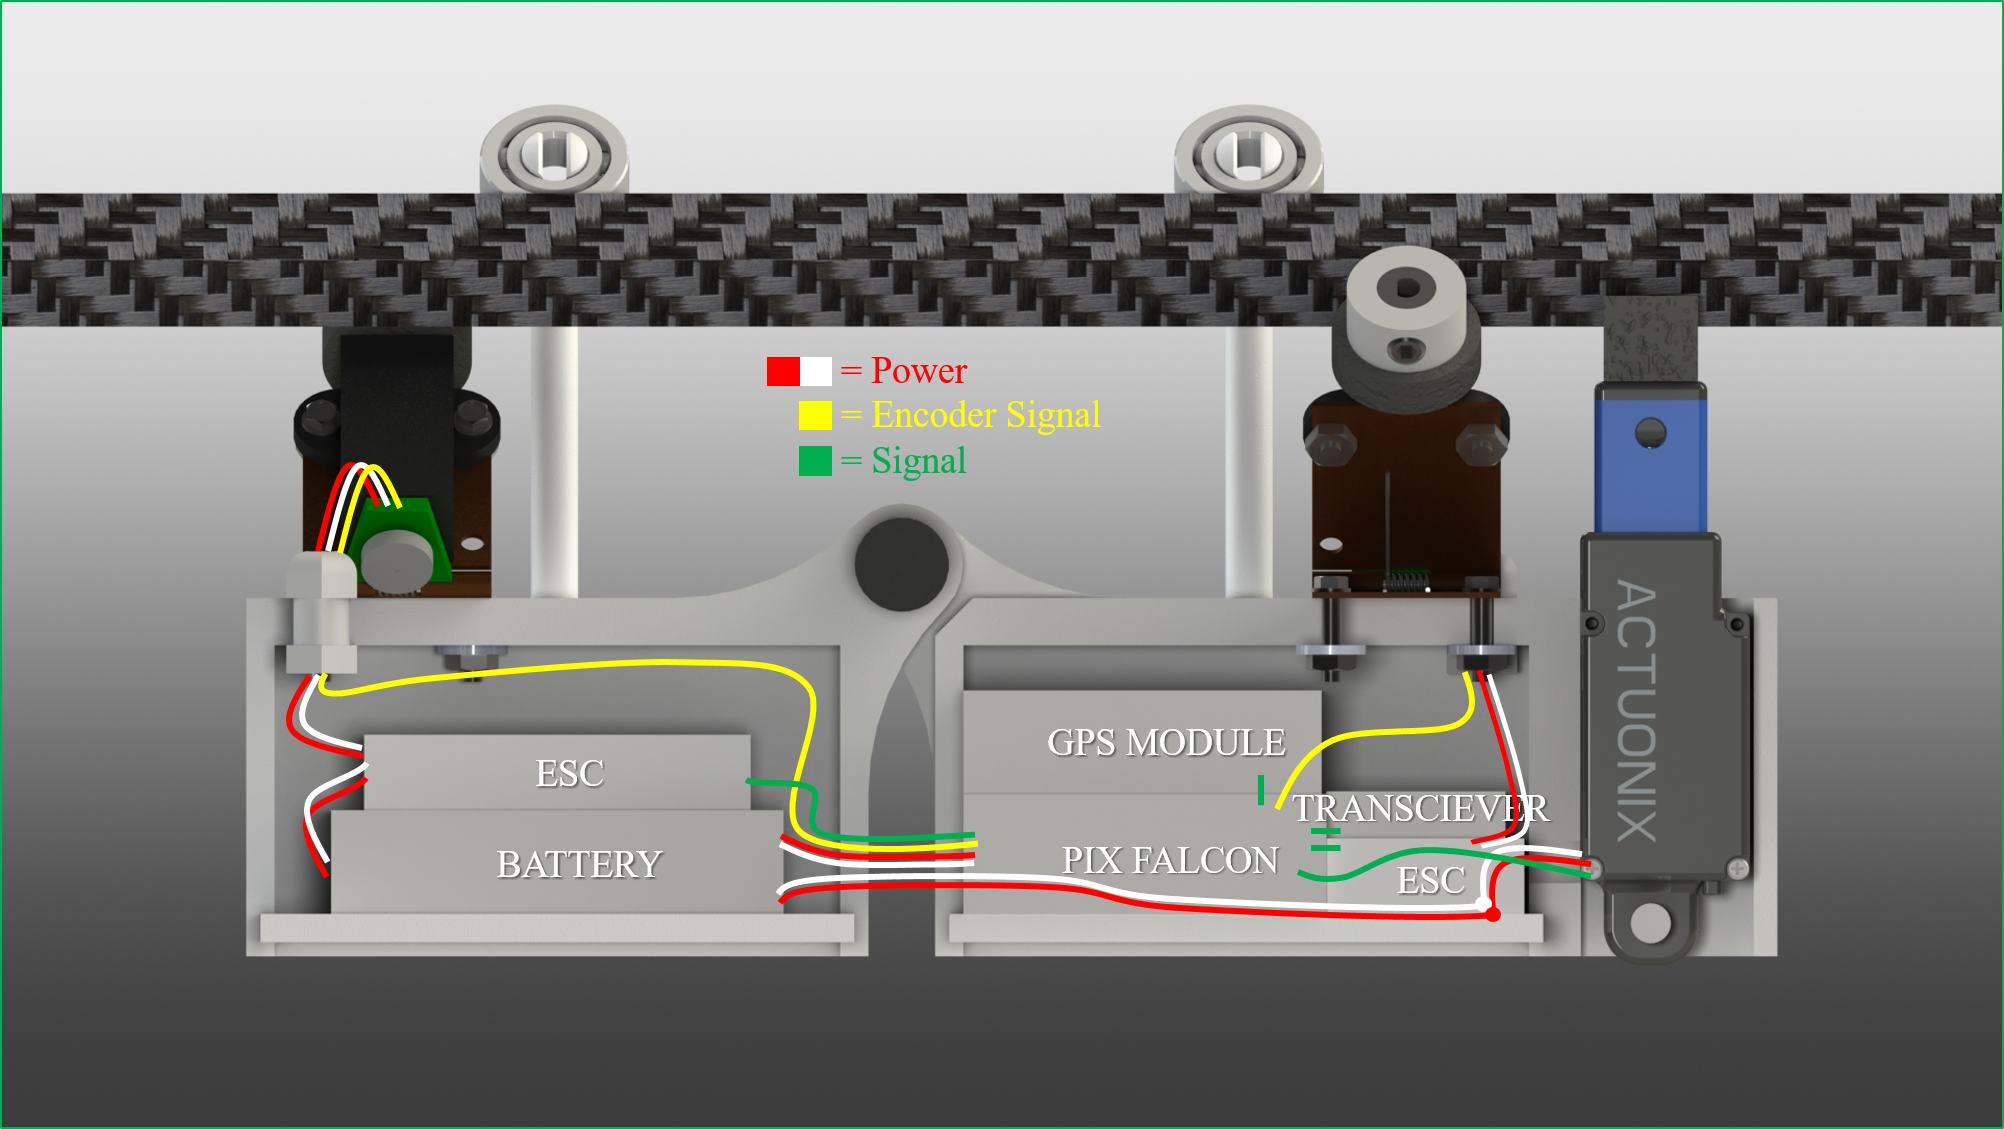
\includegraphics[width=.8\linewidth]{img/design/gondola/gondolaWiring.png}
	\caption{Gondola Component Wiring}
	\label{fig:gondolaWiring}
\end{figure}

The thruster assembly is wired similarly to the gondola, with wires coming out of the component casing. The wire is then routed through the thruster shaft. Figure \ref{fig:thrusterWiring} shows a diagram of the thruster wiring. Waterproof cannot be completed for the propeller motor as it must be exposed to the air to work effectively. Although the propeller motor is not waterproofed, it is cover by falling rain from the propeller encasement in forward flight operations.

\begin{figure}[H]
	\centering
	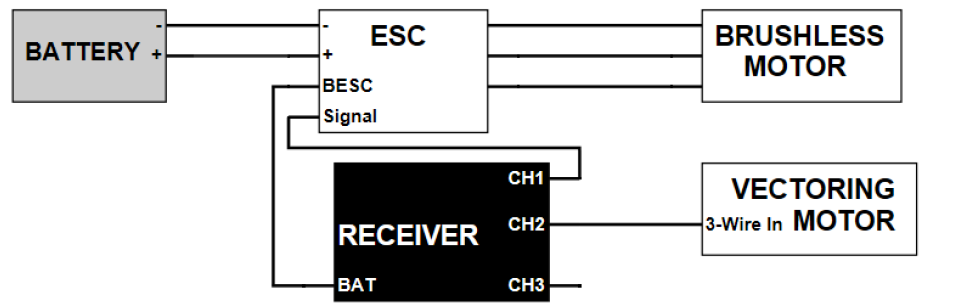
\includegraphics[width=.8\linewidth]{img/design/thruster/thrusterWiringSchematic.png}
	\caption{Thruster Wiring}
	\label{fig:thrusterWiringSchematic}
\end{figure}

\begin{figure}[H]
	\centering
	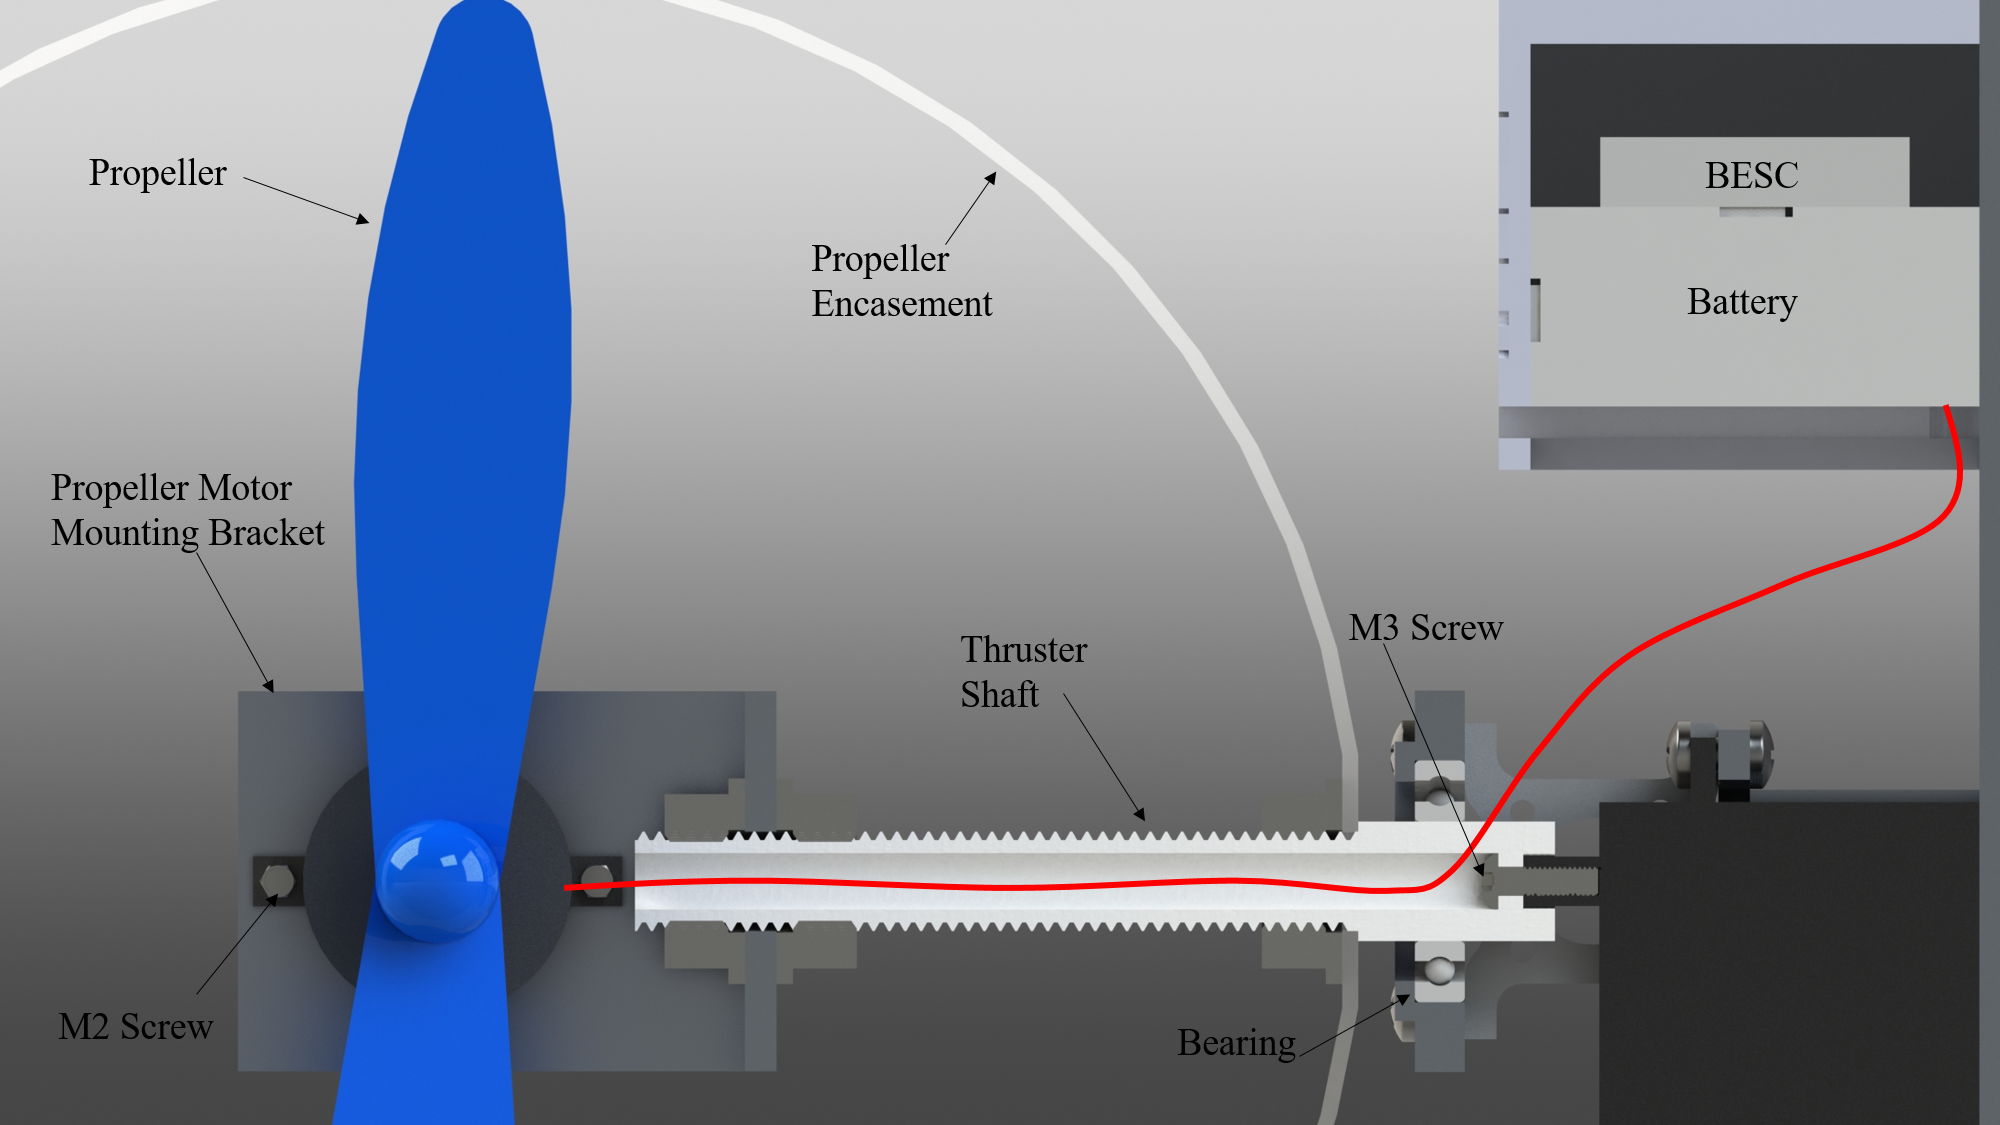
\includegraphics[width=.8\linewidth]{img/design/thruster/thrusterWiring.png}
	\caption{Thruster Wiring}
	\label{fig:thrusterWiring}
\end{figure}

\end{document}
